\documentclass{book}
\usepackage[german]{babel}
\usepackage{amsmath,amssymb,graphicx,enumerate,mathrsfs,xcolor,latexsym,theorem}

%%%%%%%%%% Start TeXmacs macros
\catcode`\<=\active \def<{
\fontencoding{T1}\selectfont\symbol{60}\fontencoding{\encodingdefault}}
\newcommand{\assign}{:=}
\newcommand{\backassign}{=:}
\newcommand{\mathLaplace}{\Delta}
\newcommand{\mathd}{\mathrm{d}}
\newcommand{\nobracket}{}
\newcommand{\textdots}{...}
\newcommand{\tmcolor}[2]{{\color{#1}{#2}}}
\newcommand{\tmdummy}{$\mbox{}$}
\newcommand{\tmop}[1]{\ensuremath{\operatorname{#1}}}
\newcommand{\tmtextbf}[1]{\text{{\bfseries{#1}}}}
\newcommand{\tmtextit}[1]{\text{{\itshape{#1}}}}
\newenvironment{enumeratealpha}{\begin{enumerate}[a{\textup{)}}] }{\end{enumerate}}
\newenvironment{enumerateroman}{\begin{enumerate}[i.] }{\end{enumerate}}
\newenvironment{itemizedot}{\begin{itemize} \renewcommand{\labelitemi}{$\bullet$}\renewcommand{\labelitemii}{$\bullet$}\renewcommand{\labelitemiii}{$\bullet$}\renewcommand{\labelitemiv}{$\bullet$}}{\end{itemize}}
\newenvironment{itemizeminus}{\begin{itemize} \renewcommand{\labelitemi}{$-$}\renewcommand{\labelitemii}{$-$}\renewcommand{\labelitemiii}{$-$}\renewcommand{\labelitemiv}{$-$}}{\end{itemize}}
\newenvironment{proof}{\noindent\textbf{Proof\ }}{\hspace*{\fill}$\Box$\medskip}
\newtheorem{corollary}{Corollary}
\newtheorem{definition}{Definition}
\newcounter{nndefinition}
\def\thenndefinition{\unskip}
\newtheorem{definition*}[nndefinition]{Definition}
{\theorembodyfont{\rmfamily}\newtheorem{example}{Example}}
\newcounter{nnexample}
\def\thennexample{\unskip}
{\theorembodyfont{\rmfamily}\newtheorem{example*}[nnexample]{Example}}
\newtheorem{lemma}{Lemma}
\newcommand{\nonconverted}[1]{\mbox{}}
\newcounter{nnremark}
\def\thennremark{\unskip}
{\theorembodyfont{\rmfamily}\newtheorem{remark*}[nnremark]{Remark}}
\newtheorem{theorem}{Theorem}
%%%%%%%%%% End TeXmacs macros

%


\begin{document}





\

\chapter{PDEs: Klassische L{\"o}sungstheorie \& Finite-Differenzen-Verfahren}

\tmtextbf{Wichtige Beispiele f{\"u}r PDEs}

Seien $\Omega \subseteq \mathbb{R}^2$, $\Omega_T \subseteq \mathbb{R} \times
\mathbb{R}^+$ Gebiete und $u \in C^2 (\Omega \rightarrow \mathbb{R})$.

Man erhalten
\begin{itemizedot}
  \item {\underline{\tmtextit{Poisson-Gleichung}}}
  
  F{\"u}r ein $f : \mathbb{R}^2 \rightarrow \mathbb{R}$ und $\forall (x, y)
  \in \Omega$:
  \[ - \frac{\partial^2}{\partial x^2} u (x, y) - \frac{\partial^2}{\partial
     y^2} u (x, y) = f (x, y) \]
  wobei $- \frac{\partial^2}{\partial x^2} u (x, y) -
  \frac{\partial^2}{\partial y^2} u (x, y)$ mit $\mathLaplace (\bullet) =
  \nabla^2 (\bullet) \assign \langle \nabla, \nabla (\bullet) \rangle $ dem
  Laplace-Operator vereinfacht wird, also $- \frac{\partial^2}{\partial x^2} u
  (x, y) - \frac{\partial^2}{\partial y^2} u (x, y) = - \Delta u$, und somit \
  \[ - \Delta u = f. \]
  \item {\underline{\tmtextit{Instation{\"a}re W{\"a}rmeleitungsgleichung /
  Diffusionsgleichung}}}
  
  F{\"u}r ein $f : \mathbb{R}^2 \rightarrow \mathbb{R}$ und $\forall (x, t)
  \in \Omega_T$:
  \[ \frac{\partial }{\partial t } u (x, t) - \frac{\partial^2}{\partial x^2}
     u (x, t) = f (x, t) . \]
  \item {\underline{\tmtextit{Wellengleichung}}}
  
  F{\"u}r $\forall (x, t) \in \Omega_T$:
  \[ \frac{\partial^2}{\partial t^2} u (x, t) = c \frac{\partial^2}{\partial
     x^2} u (x, t) . \]
\end{itemizedot}
\[ \  \]
\tmtextbf{Fragen in Kapitel 2 \& 3}
\begin{itemizedot}
  \item Gegeben eine PDE, unter welchen zus{\"a}tzlichen Bedingungen und in
  welchen Funktionenr{\"a}umen kann Existenz und Eindeutigkeit der L{\"o}sung
  garantiert werden?
  
  \item Kann f{\"u}r Spezialf{\"a}lle die L{\"o}sung explizit angegeben
  werden?
  
  \item Welche Eigenschaften haben die L{\"o}sungen? Welche Regularit{\"a}t?
  Gilt Beschr{\"a}nktheit? Gibt es Invarianzen?
  
  \item Durch welche numerische Verfahren k{\"o}nnen wir die L{\"o}sung
  approximieren?
  
  \item Konvergiert die L{\"o}sung des numerischen Verfahrens gegen die
  L{\"o}sung der PDE? Mit welcher Rate?
  
  \item Kann der Fehler der numerischen L{\"o}sung quantifiziert werden?
  
  \item Wie k{\"o}nnen numerische Verfahren effizient im Rechner umgesetzt
  werden? 
\end{itemizedot}

\section{Grundlagen / Notationen}

\begin{definition}
  \tmtextbf{(Multiindex \& Partielle Ableitung)}
  
  \tmtextit{Sei $u : \mathbb{R}^d \rightarrow \mathbb{R}$ gen{\"u}gend oft
  differenzierbar.
  
  Wir nennen $\beta = (\beta_i)_{i = 1}^d \in \mathbb{N}_0^d$ mit L{\"a}nge
  $| \beta | \assign \sum_{i = 1}^d \beta_i \backassign k$ einen
  {\underline{Multiindex der Ordnung $k$}}.
  
  Wir definieren {\underline{die partielle Ableitung von $u$ zum Index
  $\beta$}} als
  \[ \partial^{\beta} u \assign \left( \frac{\partial}{\partial x_1}
     \right)^{\beta_1} \cdots \left( \frac{\partial}{\partial x_d}
     \right)^{\beta_d} u. \]
  {\hspace{1.7em}}Dazu schreiben wir $\mathbb{B}_k \assign \{ \beta \in
  \mathbb{N}_0^d : | \beta | = k \}$ als die {\underline{Menge der
  Multiindices der Ordnung $k$}} und setze
  \[ D^k u \assign (\partial^{\beta} u)_{\beta \in \mathbb{B}_k} \]
  als den {\underline{Vektor aller partiellen Ableitungen der Ordnung $k$}}
  (mit beliebiger Reihenfolge). \ }
\end{definition}

Wir spezifieren noch einige Funktionsr{\"a}ume:

\begin{definition}
  \tmtextbf{(R{\"a}ume stetig differenzierbarer Funktionen)}
  
  \tmtextit{Sei $\Omega \subseteq \mathbb{R}^d$ offen und beschr{\"a}nkt.
  
  F{\"u}r $m \in \mathbb{N}_0$ bezeichnen wir mit $C^m \left(
  \overline{\Omega}, \mathbb{R}^n \right)$ den {\underline{Raum der $m$-mal
  stetig differenzierbarern Funktionen von $\overline{\Omega}$ nach
  $\mathbb{R}^n$}}, d.h. f{\"u}r $i \in \{ 1, \ldots, m \}$ l{\"a}sst sich die
  $i$-te Ableitung auf $\overline{\Omega}$ stetig fortsetzen, wobei $C^0
  \left( \overline{\Omega}, \mathbb{R}^n \right)$ den Raum der stetigen
  Funktionen bedeutet.
  
  F{\"u}r $n = 1$ schreiben wir auch kurz $C^m \left( \overline{\Omega}
  \right) \assign C^m \left( \overline{\Omega}, \mathbb{R} \right)$.
  
  Auf $C^0 \left( \overline{\Omega} \right)$ definieren wir die Supremumsnorm
  \[ \forall u \in C^0 \left( \overline{\Omega} \right) : \text{\qquad} \| u
     \|_{\infty} \assign \sup_{x \in \overline{\Omega}} | u (x) | \]
  und damit eine Norm auf $C^m \left( \overline{\Omega} \right)$ durch
  \[ \forall u \in C^m \left( \overline{\Omega} \right) : \text{\qquad} \| u
     \|_{C^m \left( \overline{\Omega} \right)} \assign \sum_{\forall k \in \{
     0, \ldots, m \} \forall \beta \in \mathbb{B}_k} \| \partial^{\beta} u
     \|_{\infty} . \]}
\end{definition}

\begin{remark*}
  {\tmdummy}
  
  \begin{itemizedot}
    \item $C^m \left( \overline{\Omega} \right)$ ist ein Banachraum, d.h. ein
    vollst{\"a}ndiger normierter Raum.
    
    \item F{\"u}r $u \in C^m \left( \overline{\Omega} \right)$ ist also
    $\partial^{\beta} u \in C^{m - | \beta |} \left( \overline{\Omega}
    \right)$ und f{\"u}r $l \in \{ 0, \ldots, m \}$ gilt es f{\"u}r die $l$-te
    Ableitung $D^l u \in \left( C^{m - l} \left( \overline{\Omega} \right)
    \right)^{| \mathbb{B}_l |}$.
    
    \item F{\"u}r $u \in C^1 \left( \overline{\Omega} \right)$ vereinbaren wir
    f{\"u}r den Gradient / die Jacobi-Matrix
    \[ D^1 u \assign \nabla u = \left(\begin{array}{ccc}
         \frac{\partial}{\partial x_1} u & \cdots & \frac{\partial}{\partial
         x_d} u
       \end{array}\right)^T = (D u)^T . \]
    \item F{\"u}r $m = \infty$ setzen wir
    \[ C^{\infty} \left( \overline{\Omega} \right) \assign \bigcap_{k \in
       \mathbb{N}} C^k \left( \overline{\Omega} \right) . \]
    \item Wir werden sp{\"a}ter auch R{\"a}ume $C^m (\Omega)$ f{\"u}r offenes
    und potentiell unbeschr{\"a}nktes $\Omega \subseteq \mathbb{R}^d$
    zulassen.
    
    Dabei ist eine Norm schwer definierbar, aber man kann den Raum $C^m
    (\Omega)$ mit einer Frech{\'e}t-Metrik versehen, bzgl. deren $C^m
    (\Omega)$ vollst{\"a}ndig wird (siehe Alt, Abschnitt 1.6). 
  \end{itemizedot}
\end{remark*}

In $C^m \left( \overline{\Omega} \right)$ gibt es viele Elemente, die zwar
nicht in $C^{m + 1} \left( \overline{\Omega} \right)$ liegen, aber trotzdem
sch{\"o}ne Eigenschaften haben, wie z.B. differenzierbar an sehr vielen
Stellen. Daher ist es sinnvoll, neue Funktionsr{\"a}ume zwischen $C^m \left(
\overline{\Omega} \right)$ und $C^{m + 1} \left( \overline{\Omega} \right)$ zu
definieren:

\begin{definition}
  \tmtextbf{(H{\"o}lderr{\"a}ume)}
  
  \tmtextit{F{\"u}r $\alpha \in [0, 1]$ und $u \in C^0 \left(
  \overline{\Omega} \right)$ mit $\Omega \subseteq \mathbb{R}^d$ offen \&
  beschr{\"a}nkt definieren wir die {\underline{H{\"o}lderkonstante}}
  \[ \tmop{hoel}_{\alpha} \left( u, \overline{\Omega} \right) \assign
     \sup_{x, y \in \overline{\Omega}, x \neq y} \frac{| u (x) - u (y) |}{{\|
     x - y \|^{\alpha}} } \]
  und damit die {\underline{H{\"o}lderr{\"a}ume}} durch
  \[ C^{m, \alpha} \left( \overline{\Omega} \right) \assign \left\{ u \in C^m
     \left( \overline{\Omega} \right)  | \nobracket \forall \beta \in
     \mathbb{B}_m : \tmop{hoel}_{\alpha} \left( \partial^{\beta} u,
     \overline{\Omega} \right) < \infty \right\} . \]
  {\hspace{1.7em}}H{\"o}lderr{\"a}ume $C^{m, \alpha} \left( \overline{\Omega}
  \right)$ versehen mit der Norm
  \[ \| u \|_{C^{m, \alpha} \left( \overline{\Omega} \right)} \assign \| u
     \|_{C^m \left( \overline{\Omega} \right)} + \sum_{\beta \in \mathbb{B}_m}
     \tmop{hoel}_{\alpha} \left( \partial^{\beta} u, \overline{\Omega} \right)
  \]
  sind Banachr{\"a}ume.}
\end{definition}

\begin{remark*}
  {\tmdummy}
  
  \begin{itemizedot}
    \item Der Nachweis f{\"u}r die Vollst{\"a}ndigkeit der H{\"o}lderr{\"a}ume
    findet man bei Alt, Lemma 1.8.
    
    \item Funktionen $u \in C^{0, 1} \left( \overline{\Omega} \right)$ sind
    also Lipschitz-stetig mit Lipschitz-Konstante $L \assign \tmop{hoel}_1
    \left( u, \overline{\Omega} \right)$.
  \end{itemizedot}
\end{remark*}

\begin{theorem}
  \tmtextbf{(Schachtelung der H{\"o}lderr{\"a}ume)}
  
  \tmtextit{F{\"u}r $m \in \mathbb{N}_0$ und $0 \leqslant \hat{\alpha}
  \leqslant \alpha \leqslant 1$ gilt
  \[ C^m \left( \overline{\Omega} \right) \supseteq C^{m, \hat{\alpha}}
     \left( \overline{\Omega} \right) \supseteq C^{m, \alpha} \left(
     \overline{\Omega} \right) \supseteq C^{m + 1} \left( \overline{\Omega}
     \right) . \]}
\end{theorem}

\begin{proof}
  Die erste Inklusion $C^m \left( \overline{\Omega} \right) \supseteq C^{m,
  \hat{\alpha}} \left( \overline{\Omega} \right)$ ist klar nach Definition.
  
  Verbleibendes zeigen wir f{\"u}r $m = 0$ (f{\"u}r $m > 0$ analog mit
  Ableitungen).
  \begin{itemizedot}
    \item Zweite Inklusion:
    
    F{\"u}r $u \in C^{0, \alpha} \left( \overline{\Omega} \right)$ setze
    \[ K \assign \tmop{hoel}_{\alpha} \left( u, \overline{\Omega} \right) =
       \sup_{x, y \in \overline{\Omega}, x \neq y} \frac{| u (x) - u (y) |}{\|
       x - y \|^{\alpha}} < \infty \]
    sowie
    \[ \tmop{diam} \left( \overline{\Omega} \right) \assign \sup_{x, x' \in
       \overline{\Omega}} \| x - x' \| < \infty \]
    wobei $\tmop{diam} \left( \overline{\Omega} \right) < \infty$ wegen
    Beschr{\"a}nktheit von $\overline{\Omega}$.
    
    Dazu setze
    \[ M \assign \sup_{s \in \left( 0, \tmop{diam} \left( \overline{\Omega}
       \right) \right)} \frac{s^{\alpha}}{s^{\hat{\alpha}}} = \sup_{s \in
       \left( 0, \tmop{diam} \left( \overline{\Omega} \right) \right)}
       s^{\alpha - \hat{\alpha}} . \]
    {\hspace{1.7em}}Mit $\hat{\alpha} \leq \alpha$ und $\tmop{diam} \left(
    \overline{\Omega} \right) < \infty$ ist $M$ beschr{\"a}nkt.
    
    Somit gilt f{\"u}r jedes $x, y \in \overline{\Omega}$ mit $x \neq y$:
    \[ \frac{| u (x) - u (y) |}{\| x - y \|^{\hat{\alpha}}} = \frac{| u (x) -
       u (y) |}{\| x - y \|^{\alpha}} \cdot \frac{\| x - y \|^{\alpha}}{\| x -
       y \|^{\hat{\alpha}}} \leqslant K M \]
    und daher
    \[ \tmop{hoel}_{\hat{\alpha}} \left( u, \overline{\Omega} \right) =
       \sup_{x, y \in \overline{\Omega}, x \neq y} \frac{| u (x) - u (y) |}{\|
       x - y \|^{\hat{\alpha}}} \leqslant K M < \infty \]
    also $u \in C^{0, \hat{\alpha}} \left( \overline{\Omega} \right)$.
    
    \item  Dritte Inklusion:
    
    Analog wie oben gilt f{\"u}r jedes $x, y \in \overline{\Omega}$ mit $x
    \neq y$ \
    \[ \frac{| u (x) - u (y) |}{\| x - y \|^{\alpha}} = \frac{| u (x) - u (y)
       |}{\| x - y \|} \cdot \frac{\| x - y \|}{\| x - y \|^{\alpha}} =
       \frac{| u (x) - u (y) |}{\| x - y \|} \| x - y \|^{1 - \alpha} . \]
    {\hspace{1.7em}}Da $\alpha \leqslant 1$ und $\overline{\Omega}$
    beschr{\"a}nkt, ist $\| x - y \|^{1 - \alpha}$ beschr{\"a}nkt durch ein
    $\zeta \in \mathbb{R^+}$.
    
    Daher gilt
    \[ \tmop{hoel}_{\alpha} \left( u, \overline{\Omega} \right) = \sup_{x, y
       \in \overline{\Omega}, x \neq y} \frac{| u (x) - u (y) |}{\| x - y
       \|^{\alpha}} \leqslant \sup_{x, y \in \overline{\Omega}, x \neq y}
       \frac{| u (x) - u (y) |}{\| x - y \|} \zeta \leqslant \| u' \|_{\infty}
       \zeta \]
    wobei die letzte Ungleichung aus $u \in C^1 \left( \overline{\Omega}
    \right)$ und dem Mittelwertsatz der Differenziation folgt.
    
    Also ist $\tmop{hoel}_{\alpha} \left( u, \overline{\Omega} \right) <
    \infty$ und somit $u \in C^{0, \alpha} \left( \overline{\Omega} \right)$.
  \end{itemizedot}
\end{proof}

\begin{example*}
  \
  
  F{\"u}r $\Omega = (0, 1)$ betrachten wir $u (x) = \sqrt{x}$.
  \begin{itemizedot}
    \item Es ist $u \in C^0 \left( \overline{\Omega} \right)$ aber $u \notin
    C^1 \left( \overline{\Omega} \right)$, denn $u'$ ist nicht stetig im Punkt
    $x = 0$ fortsetzbar.
    
    \item F{\"u}r $\alpha \leq \frac{1}{2}$ ist $u \in C^{0, \alpha} \left(
    \overline{\Omega} \right)$, denn f{\"u}r $x, y \in (\nobracket$ mit
    o.B.d.A. $y < x$ gilt
    \begin{eqnarray*}
      \frac{| u (x) - u (y) |}{| | x - y | |^{\alpha}} & \leqslant &
      \frac{\sqrt{x} - \sqrt{y}}{\sqrt{x - y}}\\
      & \leqslant & \frac{\left( \sqrt{x} - \sqrt{y} \right) \left( \sqrt{x}
      + \sqrt{y} \right)}{\sqrt{x - y} \left( \sqrt{x} + \sqrt{y} \right)}\\
      & = & \frac{x - y}{\sqrt{x - y} \left( \sqrt{x} + \sqrt{y} \right)}\\
      & = & \frac{\sqrt{x - y}}{\sqrt{x} + \sqrt{y}}\\
      & \leqslant & \frac{\sqrt{x}}{\sqrt{x}} = 1 < \infty .
    \end{eqnarray*}
    \item F{\"u}r $\alpha > \frac{1}{2}$ ist $u \notin C^{0, \alpha} \left(
    \overline{\Omega} \right)$, also auch nicht Lipschitz-stetig, denn
    \[ \tmop{hoel}_{\alpha} \left( u, \overline{\Omega} \right) = \sup_{x, y
       \in \overline{\Omega}, x \neq y} \frac{\left| \sqrt{x} - \sqrt{y}
       \right|}{| x - y |^{\alpha}} \geqslant \sup_{x \in \overline{\Omega}}
       \frac{\sqrt{x}}{x^{\alpha}} = \sup_{x \in \overline{\Omega}}
       \hspace{0.3em} x^{\frac{1}{2} - \alpha} = \infty . \]
  \end{itemizedot}
\end{example*}

Wir definieren hier noch die f{\"u}r sp{\"a}ter n{\"u}tzlichen R{\"a}ume:

\begin{definition}
  \tmtextbf{($L^p$-R{\"a}ume, Teil 1)}
  
  \tmtextit{Sei $\Omega \subseteq \mathbb{R}^d$ offen, beschr{\"a}nkt und
  versehen mit der gew{\"o}hnlichen Borel-$\sigma$-Algebra und dem
  $d$-dimensionalen Lebesgue-Ma{\ss} $\lambda^d$. }
  
  \tmtextit{F{\"u}r $p \in [1, \infty)$ definieren wir
  \[ \tilde{L}^p (\Omega) \assign \left\{ u : \Omega \rightarrow \mathbb{R}
     \enspace | \nobracket u \text{ ist } \lambda \text{-messbar} \wedge
     \int_{\Omega} | u |^p  \upright{d} \lambda^d < \infty \right\} \]
  und darauf eine Seminorm $\| \bullet \|_p$ durch
  \[ \| u \|_p = \| u \|_{L^p} \assign \left( \int_{\Omega} | u |^p 
     \upright{d} \lambda^d \right)^{\frac{1}{p}} . \]
  {\hspace{1.7em}}F{\"u}r $p = \infty$ definieren wir
  \[ \tilde{L}^{\infty} (\Omega) \assign \left\{ u : \Omega \rightarrow
     \mathbb{R} \enspace | \nobracket u \text{$\text{ist } \lambda
     \text{-messbar}$} \wedge \enspace \tmop{ess} \sup_{x \in \Omega} | u (x)
     | < \infty \right\} \]
  und darauf eine Norm $\| \bullet \|_{\infty}$ durch
  \[ \| u \|_{\infty} = \| u \|_{L^{\infty}} \assign \tmop{ess} \sup_{x \in
     \Omega} | u (x) | . \]}
\end{definition}

\begin{remark*}
  {\tmdummy}
  
  \begin{itemizedot}
    \item F{\"u}r $u$ messbar ist $\tmop{ess} \sup_{x \in \Omega} | u (x) | :
    = \sup_{N \subseteq \Omega, \lambda (N) = 0} \sup_{x \in \Omega \backslash
    N} | u (x) |$.
    
    \item F{\"u}r $p \in [1, \infty)$ ist $\| \bullet \|_p$ keine Norm auf
    $\tilde{L}^p (\Omega)$, denn positive Definitheit ist verletzt: F{\"u}r
    eine nicht leere Nullmenge $N \subseteq \Omega$ ist ihre charakteristische
    Funktion $\chi_N \neq 0$ aber $\| \chi_N \|_p = 0$.
    
    \item F{\"u}r $u \in C^0 \left( \overline{\Omega} \right)$ ist $u \in
    \tilde{L}^{\infty} (\Omega)$ und beide Definitionen von $\| \bullet
    \|_{\infty}$ stimmen dann {\"u}berein. 
  \end{itemizedot}
\end{remark*}

\begin{definition*}
  \tmtextbf{($L^p$-R{\"a}ume, Teil 2)}
  
  \tmtextit{Sei $\sim$ eine {\"A}quivalenzrelation auf $\tilde{L}^p (\Omega)$
  via
  \[ u \sim v \quad \Leftrightarrow \text{\quad} \exists N \subseteq \Omega
     \text{ mit } \lambda (N) = 0 \forall x \in \Omega \backslash N : u (x) =
     v (x) . \]
  {\hspace{1.7em}}Dann definiert die Menge der {\"A}quivalenzrelation
  \[ L^p (\Omega) \assign \tilde{L}^p (\Omega) / \sim \]
  den \tmtextbf{$L^p$-Raum auf $\Omega$}, wobei $\| \bullet \|_p$ kostant auf
  jeder {\"A}quivalenzklasse ist, also kann $\| \bullet \|_p$ sinnvoll auf
  $L^p (\Omega)$ erweitert werden. }
\end{definition*}

\begin{remark*}
  {\tmdummy}
  
  \begin{itemizedot}
    \item $L^p (\Omega)$ ist normierter Raum mit Norm $\| \bullet \|_p$ und
    sogar vollst{\"a}ndig, also ein Banachraum (Lemma 1.11, Satz 1.14 in Alt).
    
    \item Elemente von $L^p (\Omega)$ sind also {\"A}quivalenzklassen von
    Funktionen, die sich nur auf Nullmengen unterscheiden. Konsequente
    Unterscheidung zwischen Funktionen / {\"A}quivalenzklassen w{\"a}re sehr
    m{\"u}hsam / umst{\"a}ndlich: ,,$u \in L^p (\Omega)$`` soll eigentlich
    ,,$u \in U \in L^p (\Omega)$ f{\"u}r geeignete {\"A}quivalenzklassen $U$
    mit $u$ als Repr{\"a}sentant`` hei{\ss}en.
    
    \item {\underline{\tmtextit{Praktische Konvention}}}
    
    Wir nennen $L^p (\Omega)$ trotzdem einen Funktionenraum.
    
    Beim Arbeiten mit solchen ,,$L^p$-Funktionen`` muss jedoch immer bedacht /
    hinterfragt werden, ob Operationen sinnvoll auf $L^p (\Omega)$ definiert
    sind, d.h. {\underline{\tmtextit{ob es unabh{\"a}ngig von der Wahl des
    Repr{\"a}sentanten ist}}}.
    
    Beispiele:
    \begin{itemizeminus}
      \item Der {\underline{\tmtextit{Integraloperator}}}
      \[ T : L^1 (\Omega) \rightarrow \mathbb{R}, u \mapsto \int_{\Omega} u
         \upright{d} \lambda^d \]
      ist ein {\underline{\tmtextit{wohldefiniertes}}} stetiges lineares
      Funktional.
      
      \item {\underline{\tmtextit{Punktauswertung}}} bzgl. eines festen
      $\overline{x} \in \Omega$, also
      \[ S : L^p (\Omega) \rightarrow \mathbb{R}, u \mapsto u \left(
         \overline{x} \right) \]
      ist {\underline{\tmtextit{nicht sinnvoll definiert}}}. 
    \end{itemizeminus}
    \item Auf $L^2 (\Omega)$ ist ein Skalarprodukt $(\bullet, \bullet)$
    definiert durch
    \[ (u, v) = \langle u, v \rangle_{L^2} \assign \int_{\Omega} u v
       \upright{d} \lambda^d \]
    und dies induziert auch die $L^2$-Norm durch $\| u \| = \sqrt{(u, u)}$.
    Somit besitzt $L^2 (\Omega)$ sogar eine Hilbertraum-Struktur.
    
    \item Zu Banachraum $V$ ist der Dualraum $V'$ definiert durch
    \[ V' \assign \left\{ \varphi : V \rightarrow \mathbb{R}  | \nobracket
       \varphi \text{ist linear und stetig} \right\} \]
    und mit der induzierten Norm
    \[ \| \varphi \|_{V'} \assign \sup_{u \in V \backslash \{ 0 \}} \frac{|
       \varphi (u) |}{\| u \|_V} \]
    ist $V'$ wieder ein Banachraum.
    
    \item F{\"u}r $1 < p, q < \infty$ mit $\frac{1}{p} + \frac{1}{q} = 1$ ist
    $L^q (\Omega)$ isomorph zu $(L^p (\Omega))^{'}$.
    
    \item $L^2 (\Omega)$ ist also wegen $\frac{1}{2} + \frac{1}{2} = 1$
    isomorph zu seinem eigenen Dualraum. 
  \end{itemizedot}
\end{remark*}

\begin{theorem}
  \tmtextbf{(Young'sche Ungleichung)}
  
  \tmtextit{Seien $a, b \in \mathbb{R}_+$ und $p, q \in (1, \infty)$ mit
  $\frac{1}{p} + \frac{1}{q} = 1$.
  
  Dann gilt
  \[ a b \leqslant \frac{1}{p} a^p + \frac{1}{q} b^q . \]}
\end{theorem}

\begin{proof}
  F{\"u}r $a = b = 0$ ist die Behauptung klar, daher seien $a \neq 0 \neq b$.
  
  Die Konkavit{\"a}t des Logarithmus liefert
  \[ \ln (a b) = \ln (a) + \ln (b) = \frac{1}{p} \ln (a^p) + \frac{1}{q} \ln
     (b^q) \leqslant \ln \left( \frac{1}{p} a^p + \frac{1}{q} b^q \right) . \]
  {\hspace{1.7em}}Anwendung von $\exp$ auf beiden Seiten liefert die
  Behauptung. 
\end{proof}

\begin{corollary}
  \tmtextbf{(Young'sche Ungleichung f{\"u}r $p = q = 2$)}
  
  \tmtextit{F{\"u}r $a, b \in \mathbb{R}_+$ und beliebiges $\varepsilon \in
  \mathbb{R}_+$ gilt
  \[ a b \leqslant \frac{\varepsilon}{2} a^2 + \frac{1}{2 \varepsilon} b^2 .
  \]}
\end{corollary}

\begin{remark*}
  {\tmdummy}
  
  \begin{itemizedot}
    \item Beweis von 2.7 durch $a b = \left( \sqrt{\varepsilon} a \right)
    \left( \frac{1}{\sqrt{\varepsilon}} b \right)$ und dann Anwendung von 2.6.
    
    \item 2.7 wird h{\"a}ufig verwendet um ,,Produkte zu Spalten`` und einen
    Term beliebig klein zu machen durch geeignetes $\varepsilon$. 
  \end{itemizedot}
\end{remark*}

\begin{theorem}
  \tmtextbf{(H{\"o}lder-Ungleichung)}
  
  \tmtextit{Seien $p, q \in [1, \infty]$ mit $\frac{1}{p} + \frac{1}{q} = 1$,
  $u \in L^p (\Omega)$ und $v \in L^q (\Omega)$ beliebig.
  
  Dann ist das Produkt $u v \in L^1 (\Omega)$ und es gilt
  \[ \| u v \|_1 \leqslant \| u \|_p \| v \|_q . \]}
\end{theorem}

\begin{remark*}
  {\tmdummy}
  
  \begin{itemizedot}
    \item Den Beweis von 2.8 {\"u}berlassen wir als {\"U}bung.
    
    \item F{\"u}r $p = q = 2$ folgt die Cauchy-Schwarz-Ungleichung
    \[ | (u, v) | = \left| \int_{\Omega} u v \upright{d} \lambda^d \right|
       \leqslant \int_{\Omega} | u v |  \upright{d} \lambda^d = \| u v \|_1
       \leqslant \| u \|_2 \| v \|_2 = \sqrt{(u, u)} \sqrt{(v, v)} . \]
  \end{itemizedot}
\end{remark*}

\begin{definition}
  \tmtextbf{(Lokal integrierbare Funktionen)}
  
  \tmtextit{Wir definieren den Raum der {\underline{lokal integrierbaren
  Funktionen}}
  \[ L^1_{\tmop{loc}} (\Omega) \assign \left\{ u : \Omega \rightarrow
     \mathbb{R}  | \nobracket u \text{ Lebesgue-messbar} \enspace \wedge
     \text{\enspace} \forall K \subseteq \Omega \text{kompakt:} \int_K | u |
     \upright{d} \lambda^d < \infty \right\} . \]}
\end{definition}

\begin{example*}
  {\tmdummy}
  
  \begin{itemizedot}
    \item $u \in L^1 (\Omega)${\hspace{1.7em}}$\Rightarrow$\quad$u \in
    L^1_{\tmop{loc}} (\Omega)$.
    
    \item $u \in L^1_{\tmop{loc}} (\Omega)$\quad$\nRightarrow$\quad$u \in L^1
    (\Omega)$, z.B. $u \equiv 1$ liegt in $L^1_{\tmop{loc}} (\Omega)$ aber
    nicht in $L^1 (\Omega)$.
  \end{itemizedot}
\end{example*}

\begin{definition}
  \tmtextbf{(Funktionen mit kompaktem Tr{\"a}ger)}
  
  \tmtextit{F{\"u}r $\Omega \in \mathbb{R}^d$ offen (aber m{\"o}glicherweise
  unbeschr{\"a}nkt) und $m \in \mathbb{N_0 \cup \{ \infty \}}$ definieren wir
  \
  \[ C^m_0 (\Omega) \assign \left\{ u \in C^m (\Omega)  | \nobracket
     \tmop{supp} (u) \subseteq \Omega \text{ kompakt} \right\} \]
  wobei $\tmop{supp} (u) \assign \overline{\{ x \in \Omega | \nobracket u (x)
  \neq 0 \}}$ den {\underline{Tr{\"a}ger}} von $u$ bedeutet.}
\end{definition}

\begin{theorem}
  \tmtextbf{(Fundamentallemma der Variationsrechnung)}
  
  \tmtextit{F{\"u}r $\Omega \subseteq \mathbb{R}^d$ offen und $u \in
  L^1_{\tmop{loc}} (\Omega)$} gilt
  \[ \forall v \in C^{\infty}_0 (\Omega) : \int_{\Omega} u v \upright{d}
     \lambda^d = 0 \quad \Leftrightarrow \text{\quad} u = 0 \text{fast
     {\"u}berall} . \]
\end{theorem}

Wir verweisen auf 2.11 in Alt f{\"u}r den Beweis von 2.11.

\begin{definition}
  \tmtextbf{(Ableitungsoperatoren)}
  
  \tmtextit{Sei $\Omega \subseteq \mathbb{R}^d$. F{\"u}r $i \in \{ 1, \ldots,
  d \}$ schreiben wir $\partial_{x_i} \assign \frac{\partial}{\partial x_i}$.
  \
  
  F{\"u}r $u \in C^1 (\Omega)$ definieren wir den {\underline{Gradienten}}
  von $u$ durch
  \[ \tmop{grad} u = \nabla u \assign \left(\begin{array}{c}
       \partial_{x_1} u\\
       \vdots\\
       \partial_{x_d} u
     \end{array}\right) . \]
  {\hspace{1.7em}}F{\"u}r Vektorfeld $v = (v_i)_{i = 1}^d \in C^1 (\Omega,
  \mathbb{R}^d)$ definieren wir die {\underline{Divergenz}}
  \[ \tmop{div} v \assign \nabla \bullet v = \sum_{i = 1}^d \partial_{x_i}
     v_i \]
  und f{\"u}r $d = 3$ die {\underline{Rotation}} \
  \[ \tmop{rot} v \assign \nabla \times v = \left(\begin{array}{c}
       \partial_{x_2} v_3 - \partial_{x_3} v_2\\
       \partial_{{x_3} } v_1 - \partial_{x_1} v_3\\
       \partial_{{x_1} } v_2 - \partial_{{x_2} } v_1
     \end{array}\right) . \]
  {\hspace{1.7em}}F{\"u}r $u \in C^2 (\Omega)$ definieren wir den
  {\underline{Laplace-Operator}} durch
  \[ \mathLaplace u \assign \nabla \bullet (\nabla u) = \tmop{div}
     \tmop{grad} u = \sum_{i = 1}^d \partial_{x_i }^2 u = \tmop{Spur} (H u) \]
  wobei $H u$ die Hesse-Matrix von $u$ bezeichnet.}
\end{definition}

\begin{definition}
  \tmtextbf{(Lipschitz-Gebiet)}
  
  \tmtextit{Sei $\Omega \subseteq \mathbb{R}^d$ offen und beschr{\"a}nkt.
  
  $\Omega$ hei{\ss}t {\underline{Lipschitz-Gebiet}} g.d.w. es endlich viele
  offene Menge $U_1, \ldots, U_n \subseteq \mathbb{R}^d$ existieren, s.d. die
  folgenden zwei Bedingungen erf{\"u}llt werden:
  \begin{itemizedot}
    \item Der Rand von $\Omega$ wird durch $U_1, \ldots, U_d$ {\"u}berdeckt,
    also $\partial \Omega \subseteq \bigcup_{i = 1}^n U_i$, und
    
    \item $\forall i \in \{ 1, \ldots, n \} : \partial \Omega \cap U_i$
    l{\"a}sst sich in geeigneter Richtung als Graph einer Lipschitz-stetigen
    Funktion schreiben und $\Omega$ liegt auf einer Seite des Graphen.
  \end{itemizedot}}
\end{definition}

\begin{example*}
  \
  
  Gegeben z.B. folgende zwei Gebiete.
  \[ 
     \raisebox{-0.00249573482817451\height}{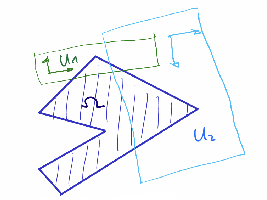
\includegraphics[width=4.47904368358914cm,height=3.36399711399711cm]{k2-1.pdf}}
     \hspace{4em}
     \raisebox{-0.00255272473450666\height}{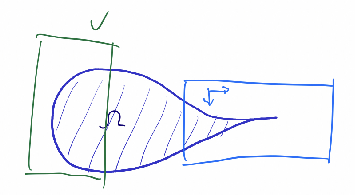
\includegraphics[width=5.96645021645022cm,height=3.28889544798636cm]{k2-2.pdf}}
  \]
  {\hspace{1.7em}}Das linke Gebiet ist ein Lipschitz-Gebiet.
  
  Das rechte Gebiet ist kein Lipschitz-Gebiet, denn dabei l{\"a}sst sich die
  ,,Spitze`` nicht als Lipschitz-stetige Funktion darstellen. 
\end{example*}

\begin{theorem}
  \tmtextbf{(Satz von Gau{\ss} f{\"u}r Lipschitz-Gebiet)}
  
  \tmtextit{Sei $\Omega \subseteq \mathbb{R}^d$ Lipschitz-Gebiet und $v \in
  C^0 \left( \overline{\Omega}, \mathbb{R}^d \right) \cap C^1 (\Omega,
  \mathbb{R}^d)$ ein Vektorfeld mit $\tmop{div} v \in L^1 (\Omega)$, d.h. auf
  $\partial \Omega$ ist $v$ zwar nicht differenzierbar, aber $v$ bleibt
  beschr{\"a}nkt.
  
  Dann gilt
  \[ \int_{\Omega} \tmop{div} v \upright{d} \lambda^d = \int_{\partial
     \Omega} v \bullet n \upright{d} \lambda^{d - 1} \]
  wobei $n : \mathbb{R}^d \rightarrow \mathbb{R}^d$ {\"a}u{\ss}ere
  Einheitsnormale an den Rand von $\Omega$ bezeichnet. }
\end{theorem}

Wir verweisen auf A.5.9. in Alt f{\"u}r den Beweis von 2.14, und nutzen dies
direkt um eine vektorielle Form von partieller Integration zu formulieren:

\begin{corollary}
  \tmtextbf{(Partielle Integration)}
  
  \tmtextit{F{\"u}r $u \in C^1 \left( \overline{\Omega} \right)$ und $v \in
  C^1 \left( \overline{\Omega}, \mathbb{R}^d \right)$ gilt
  \[ \int_{\Omega} \nabla u \bullet v \upright{d} \lambda^d = - \int_{\Omega}
     u \tmop{div} v \upright{d} \lambda^d + \int_{\partial \Omega} u v \bullet
     n \upright{d} \lambda^{d - 1} . \]}
\end{corollary}

\begin{proof}
  Satz von Gau{\ss} 2.14 \& Produktregel liefern:
  \[ \int_{\partial \Omega} u v \bullet n \upright{d} \lambda^{d - 1} =
     \int_{\Omega} \tmop{div} (u v)  \upright{d} \lambda^d = \int_{\Omega}
     \nabla u \bullet v \upright{d} \lambda^d + \int_{\Omega} u \tmop{div} v
     \upright{d} \lambda^d \]
\end{proof}

Nachdem wir die funktionaltheoretischen Grundlagen gesammelt haben,
formulieren wir jetzt die Gegenst{\"a}nde, f{\"u}r die wir uns eigentlich
interessieren:

\begin{definition}
  \tmtextbf{(Skalare PDE)}
  
  \tmtextit{Sei $k \in \mathbb{N}$, $\Omega \subseteq \mathbb{R}^d$ und $F :
  \mathbb{R}^{| \mathbb{B}_k |} \times \mathbb{R}^{| \mathbb{B}_k - 1 |}
  \times \cdots \times \mathbb{R}^d \times \mathbb{R} \times \Omega
  \rightarrow \mathbb{R}$.
  
  Wir nennen
  \begin{equation}
    \forall x \in \Omega : \text{\quad} F (D^k u (x), D^{k - 1} u (x), \ldots,
    D^1 u (x), u (x), x) = 0
  \end{equation}
  eine {\underline{skalare PDE der Ordnung $k$}} f{\"u}r die unbekannte
  L{\"o}sung $u : \Omega \rightarrow \mathbb{R}$. \ }
\end{definition}

Es gibt auch Systeme von PDEs f{\"u}r vektorielle Funktionen, aber wir
betrachten sie hier nicht.

\begin{definition}
  \tmtextbf{(Klassisiche L{\"o}sung)}
  
  \tmtextit{Sei eine skalare PDE gem{\"a}{\ss} (2.1) gegeben.
  
  Falls eine Funktion $u \in C^k (\Omega)$ die Bedingung (2.1) erf{\"u}llt,
  dann nennen wir $u$ eine {\underline{klassische L{\"o}sung}} der PDE. \ }
\end{definition}

Im Kapitel 2 besch{\"a}ftigen wir uns mit klassischer L{\"o}sung und im
Kapitel 3 werden wir sehen, warum dieser Begriff in vielen F{\"a}llen zu
eingeschr{\"a}nkt ist.

\

Als n{\"a}chstes f{\"u}hren wir noch einige wichtigen Arten von PDEs ein, und
diese Begriffe bezeichnet man oft als \tmtextbf{Klassifikation linearer PDEs
zweiter Ordnung}.

\begin{definition}
  \tmtextbf{(Linearer Differenzialoperator 2. Ordnung)}
  
  \tmtextit{Sei $\Omega \in \mathbb{R}^d$ offen, }$A = (a_{i j})_{i, j = 1}^d
  \in C^0 (\Omega, \mathbb{R}^{d \times d})$, $b = (b_i)_{i = 1}^d \in C^0
  (\Omega, \mathbb{R}^d)$ \tmtextit{\&} $c \in C^0 (\Omega)$.
  
  \tmtextit{Dann nennen wir $\mathscr{L} : C^2 (\Omega) \rightarrow C^0
  (\Omega)$ mit}
  \[ (\mathscr{L} u) (x) = - \sum_{i, j = 1}^d a_{i j} (x) \partial_{x_i}
     \partial_{x_j} u (x) + \sum_{i = 1}^d b_i (x) \partial_{x_i} u (x) + c
     (x) u (x) \]
  \tmtextit{einen {\underline{linearen Differenzialoperator zweiter Ordnung}}.
  }
\end{definition}

\begin{remark*}
  {\tmdummy}
  
  \begin{itemizedot}
    \item Mit  L  werden $u$ sowie die m{\"o}glichen 1. \& 2. partiellen
    Ableitungen von $u$ mit skalarwertigen Funktionen multipliziert und dann
    addiert.
    
    \item Wir nennen $- \sum_{i, j = 1}^d a_{i j} (x) \partial_{x_i}
    \partial_{x_j} u (x)$ den {\underline{\tmtextit{Hauptteil von
    $\mathscr{L}$}}}.
    
    \item OBdA kann $A$ symmetrisch gew{\"a}hlt werden, denn $\partial_{x_i}
    \partial_{x_j} = \partial_{x_j} \partial_{x_i}$, also falls $A$ nicht
    symmetrisch ist, ergibt $\tilde{A} \assign \frac{1}{2} (A + A^T)$
    identisches $\mathscr{L}$.
    
    \item Da $A$ oBdA symmetrisch ist, kann man annehmen, dass f{\"u}r jedes
    $x \in \Omega$, $A (x)$ nur reelle Eigenwerte hat.
    
    \item Zu $f \in C^0 (\Omega)$ ergibt sich entsprechende PDE
    \begin{equation}
      \mathscr{L} u = f.
    \end{equation}
  \end{itemizedot}
\end{remark*}

\begin{definition}
  \tmtextbf{(Klassifikation)}
  
  \tmtextit{Sei $\mathscr{L}$ ein linearer Differentialoperator zweiter
  Ordnung bzgl. $(A, b, c)$ wobei $A$ symmetrisch ist und $x \in \Omega$.
  
  Der Operator $\mathscr{L}$ hei{\ss}t
  \begin{itemizedot}
    \item {\underline{elliptisch in $x$}}, falls alle Eigenwerte von $A (x)$
    gleichzeitig positiv oder gleichzeitig negativ sind,
    
    \item {\underline{parabolisch in $x$}}, falls $d - 1$ Eigenwerte von $A
    (x)$ gleichzeitig positiv oder gleichzeitig negativ sind und einen
    Eigenwert $0$ ist, aber die Matrix $(A (x) b (x)) \in \mathbb{R}^{d + 1
    \times d}$ vollen Rang besitzt, also $\tmop{Rang} (A (x) b (x)) = d$,
    
    \item {\underline{hyperbolisch in $x$}}, falls $d - 1$ Eigenwerte von $A
    (x)$ positiv (oder alle negativ) sind und einen Eigenwert negatives (oder
    positives) Vorzeichen besitzt. 
  \end{itemizedot}
  {\hspace{1.7em}}Der Operator $\mathscr{L}$ hei{\ss}t {\underline{elliptisch
  / parabolisch / hyperbolisch in $\Omega$}}, falls er eplliptisch /
  parabolisch / hyperbolisch in allen Punkten von $\Omega$ ist.
  
  Die PDE gem{\"a}{\ss} (2.2) ist elliptisch / parabolisch / hyperbolisch,
  falls der zugeh{\"o}rige Operator $\mathscr{L}$ dies in $\Omega$ ist. }
\end{definition}

\begin{remark*}
  {\tmdummy}
  
  \begin{itemizedot}
    \item Die Klassifikation ist nicht vollst{\"a}ndig bzw. nicht
    ersch{\"o}pfend, aber ausreichend f{\"u}r die meisten praktischen Zwecke.
    
    \item In der Praxis ist auch {\"A}nderung des Typs in Teilgebieten von
    $\Omega$ m{\"o}glich, und solche PDEs nennt man ,,{\underline{vom
    gemischten Typ}}``.
    
    \item Begriffe sind motiviert aus Kegelschnitten / Quadriken
    \[ z^T A (x) z = 1, \]
    welche unter den geannten Bedingungen ein Ellipsoid, Paraboloid bzw.
    Hyperboloid beschreiben.
    
    \item In Def. 2.18 wird Zeitvariable $t$, falls vorhanden, als eine der
    Variablen $x_i$ interpretiert, d.h. auch Zeitableitung erster oder zweiter
    Ordnung erlaubt.
  \end{itemizedot}
\end{remark*}

\begin{example*}
  {\tmdummy}
  
  \begin{enumerateroman}
    \item {\underline{\tmtextit{Laplace / Poisson-Gleichung}}} ( $-
    \mathLaplace u = f$ ):
    
    Dabei ist
    \[ \mathscr{L} u = - \mathLaplace u \]
    und d.h. \
    \[ A = I, \text{\quad} b = 0, \text{\quad} c = 0. \]
    {\hspace{1.7em}}$A$ hat nur positive Eigenwerte und somit ist
    $\mathscr{L}$ elliptisch.
    
    \item {\underline{Instation{\"a}re W{\"a}rmeleitung}} ( $\partial_t u -
    \partial_x^2 u = f$ ):
    
    Dabei ist
    \[ \mathscr{L} u = \partial_t u - \partial_x^2 u \]
    und d.h.
    \[ A = \left(\begin{array}{cc}
         I & \\
         & 0
       \end{array}\right), \text{\quad} b = \left(\begin{array}{c}
         0\\
         \vdots\\
         0\\
         1
       \end{array}\right), \text{\quad} c = 0. \]
    {\hspace{1.7em}}$A$ hat $d - 1$ positive Eigenwerte und $\tmop{Rang} (A,
    b) = d$, also $\mathscr{L}$ parabolisch.
    
    \item {\underline{Wellengleichung}} ( $\partial_t^2 u - \Delta u = f$ ):
    
    Dabei ist
    \[ \mathscr{L} u = \partial_t^2 u - \Delta u \]
    und d.h.
    \[ A = \left(\begin{array}{cc}
         I & \\
         & - 1
       \end{array}\right), \text{\quad} b = 0, \text{\quad} c = 0. \]
    {\hspace{1.7em}}$A$ hat $d - 1$ positive Eigenwerte und einen negativen
    Eigenwert, also ist $\mathscr{L}$ hyperbolisch.
    
    \item {\underline{Tricomi-Gleichung}} ( $x_2 \partial_{x_1}^2 u +
    \partial_{x_2}^2 u = 0$ f{\"u}r $\Omega = \mathbb{R}^2$ ):
    
    Dabei ist
    \[ \mathscr{L} u = x_2 \partial_{x_1}^2 u + \partial_{x_2}^2 u \]
    und d.h.
    \[ A = \left(\begin{array}{cc}
         x_2 & \\
         & 1
       \end{array}\right), \text{\quad} b = 0, \text{\quad} c = 0. \]
    {\hspace{1.7em}}Also ist die Gleichung vom gemischten Typ:
    \begin{itemizedot}
      \item elliptisch in $(x_1, x_2) \in \mathbb{R} \times \mathbb{R}_+$,
      
      \item hyperbolisch in $(x_1, x_2) \in \mathbb{R} \times \mathbb{R}_-$.
    \end{itemizedot}
    {\hspace{1.7em}}Aber f{\"u}r $x_2 = 0$ ist die Gleichung nicht
    parabolisch, denn dann ist $\tmop{Rang} \left( A \enspace b \right) = 1
    \neq 2$.
  \end{enumerateroman}
\end{example*}

\begin{remark*}
  \tmtextbf{(Charakterisierung)}
  
  Unterscheidung in Typen ist sinnvoll wegen wesentlich unterschiedlichen
  L{\"o}sungseigenschaften:
  \begin{itemizedot}
    \item Elliptische PDEs:
    \begin{itemizeminus}
      \item L{\"o}sungen sind oft sehr glatt und meistens sind die
      Randbedingungen vorgegeben.
      
      \item L{\"o}sungen erf{\"u}llen h{\"a}ufig ,,Maximumsprinzip`` (dies
      wird sp{\"a}ter erkl{\"a}rt).
    \end{itemizeminus}
    \item Parabolische PDEs:
    \begin{itemizeminus}
      \item ,,Ausgezeichnete`` Achse ist meistens die Zeitachse. Die PDE kann
      oft umgeschrieben werden als
      \[ \partial_t u + \widetilde{\mathcal{\mathscr{L}}} u = \tilde{f} \]
      wobei $\widetilde{\mathcal{\mathscr{L}}}$ ein elliptischer Operator auf
      dem Raum erzeugt von den anderen $d - 1$ Eigenvektoren.
      
      \item H{\"a}ufige Anfangswerte f{\"u}r $u$ und ggf. Randwerte f{\"u}r
      $u$ vorgegeben.
      
      \item Operator hat regularisierenden Effekt, d.h. L{\"o}sungen sind
      h{\"a}ufig glatter als Anfangsdaten.
      
      \item ,,Unendliche Ausbreitungsgeschwindikeit`` kann man dabei
      beobachten.
    \end{itemizeminus}
    \item Hyperbolische PDEs:
    \begin{itemizeminus}
      \item ,,Ausgezeichnete`` Achse ist meistens die Zeitachse. Die PDE kann
      oft umgeschrieben werden als
      \[ \partial^2_t u + \widetilde{\mathcal{\mathscr{L}}} u = \tilde{f} \]
      wobei $\widetilde{\mathcal{\mathscr{L}}}$ ein elliptischer Operator
      (bzgl. $x$) mit negativen Eigenwerten ist.
      
      \item Solche PDEs beschreiben Schwingungsvorg{\"a}nge.
      
      \item Es werden Anfangsbedingungen f{\"u}r $u$ und f{\"u}r $\partial_t
      u$ vorgegeben, ggf. noch Randbedingungen f{\"u}r $u$.
      
      \item ,,Endliche Ausbreitungsgeschwindigkeit`` liegt meist vor.
      
      \item Kein regularisierender Effekt l{\"a}sst sich beobachten. \ 
    \end{itemizeminus}
  \end{itemizedot}
\end{remark*}

\begin{remark*}
  \tmtextbf{(Eigenschaften allgemeiner elliptischer Operatoren)}
  \begin{itemizedot}
    \item Falls  L  rotationsinvariant ist, dann ist $\mathcal{\mathscr{L}} u
    = - a \Delta u + c u$ f{\"u}r ein $a \in \mathbb{R}_+$, d.h. $A = a I$ und
    $b = 0$.
    
    \item Wir nennen $\mathcal{\mathscr{L}}$
    {\underline{\tmtextit{gleichm{\"a}{\ss}ig elliptisch}}}, falls $\exists
    \alpha \in \mathbb{R}_+$ s.d.
    \[ \forall z \in \mathbb{R}^d \enspace \forall x \in \Omega :
       \text{\enspace} \langle z, A (x) z \rangle \geqslant \alpha \| z \|^2,
    \]
    also sind alle Eigenwerte von $A (x)$ mind. so gro{\ss} wie $\alpha$.
    Dieses $\alpha$ nennt man
    {\underline{\tmtextit{Elliptizit{\"a}tskonstante}}}.
    
    \item F{\"u}r gleichm{\"a}{\ss}ige elliptische PDEs folgen auch Maximums,
    Minimums \& Vergleichsprinzip. Dies wird bald f{\"u}r Poisson-Gleichung
    betrachtet. 
  \end{itemizedot}
\end{remark*}

Iim Folgenden beschr{\"a}nken wir unsere Betrachtung auf eine spezielle PDE:

\

\section{Poisson-Gleichung}

\begin{definition}
  \tmtextbf{(Poisson / Laplace-Gleichung)}
  
  \tmtextit{Sei $\Omega \subseteq \mathbb{R}^d$.
  
  Wir nennen die PDE
  \[ - \Delta u = 0 \]
  {\underline{Laplace-Gleichung}}.
  
  F{\"u}r ein $f : \Omega \rightarrow \mathbb{R}$ nennen wir die PDE
  \[ - \Delta u = f \]
  die {\underline{Poisson-Gleichung}}. }
\end{definition}

\begin{remark*}
  {\tmdummy}
  
  \begin{itemizedot}
    \item Das Vorzeichen ist eigentlich willk{\"u}rlich, aber so taucht es in
    Def. 2.18 auf.
    
    \item Wir erwarten i.A. keine Eindeuktigkeit von L{\"o}sungen:
    
    Mit $u$ einer L{\"o}sung ist auch $u + c$ f{\"u}r jedes $c \in
    \mathbb{R}$ auch eine L{\"o}sung von Laplace- \& von Poisson-Gleichung.
    
    $\rightsquigarrow$ Weitere Bedingung erforderlich, also Randbedingung.
    
    \item Klassische L{\"o}sungen von $- \Delta u = 0$ nennen wir auch
    {\underline{\tmtextit{harmonisch}}}.
  \end{itemizedot}
\end{remark*}

\begin{remark*}
  \tmtextbf{(Rotations- \& Translationsinvarianz)}
  \begin{itemizedot}
    \item Falls $f$, $\Omega$ rotationssymmetrisch sind, d.h. f{\"u}r $\forall
    T \in O_d (\mathbb{R})$ gilt $\Omega = T \Omega$ und f{\"u}r $\forall x
    \in \Omega : f (x) = f (T x)$, dann liefert jede klassische L{\"o}sung der
    Poisson-Gleichung $u \in C^2 (\Omega)$ mit $T$ eine neue klassische
    L{\"o}sung, n{\"a}mlich $v : = u \circ T$.
    
    \item Falls $f$, $\Omega$ translationsinvariant bzgl. $t \in \mathbb{R}^d$
    sind, d.h. $\Omega = \Omega + t$ sowie $\forall x \in \Omega : f (x) = f
    (x + t)$, dann ist mit $u$ klassischer L{\"o}sung auch $v (x) \assign u (x
    + t)$ eine klassische L{\"o}sung der Poisson-Gleichung. 
  \end{itemizedot}
\end{remark*}

Unser \tmtextbf{Ziel} besteht darin, L{\"o}sungen der Poisson-Gleichung zu
finden und ihre Eigenschaften zu untersuchen.

Die L{\"o}sungen erhalten wir in zwei Schritten:
\begin{enumerateroman}
  \item Konstruiere f{\"u}r Laplace-Gleichung ($f = 0$) auf $\Omega \assign
  \mathbb{R}^d \backslash \{ 0 \}$ spezielle rotationssymmetrische
  L{\"o}sungen, also die sogenannten ,,Fundamentall{\"o}sungen``;
  
  \item Konstruiere f{\"u}r die Poisson-Gleichung (i.A. $f \neq 0$)
  L{\"o}sungen durch Faltung mit Fundamentall{\"o}sungen. 
\end{enumerateroman}
\begin{remark*}
  \tmtextbf{(Ansatz f{\"u}r Fundamentall{\"o}sung der Laplace-Gleichung)}
  
  Annahme von Rotationssymmetrie \& Umschreiben der PDE als ODE:
  \begin{itemizedot}
    \item Sei $u \in C^2 (\Omega)$ klassische L{\"o}sung der Laplace-GLeichung
    f{\"u}r $\Omega = \mathbb{R}^d \backslash \{ 0 \}$ rotationsinvariant,
    d.h. es existiert ein $v \in C^2 ((0, \infty))$ mit $u (x) = v (\| x
    \|_2)$.
    
    \item F{\"u}r $x \in \mathbb{R}^d$ schreiben wir $r (x) \assign \| x \|_2
    = (\langle x, x \rangle)^{\frac{1}{2}}$. Es ist also
    \[ u (x) = v (r (x)) \]
    und wir werden, wenn es keine Mehrdeutigkeit gibt, $r (x)$ mit $r$
    abgek{\"u}rzt.
    
    \item Wir sehen zun{\"a}chst
    
    
    \[ \nabla_x r = \left( (\langle x, x \rangle)^{\frac{1}{2}} \right)' =
       \frac{1}{2} (\langle x, x \rangle)^{- \frac{1}{2}}  (\langle x, x
       \rangle)' = \frac{1}{2} (\langle x, x \rangle)^{- \frac{1}{2}} 2 x =
       \frac{x}{r} \]
    wobei man $(\langle x, x \rangle)' = 2 x$ aus
    \[ \langle x + h, x + h \rangle = \langle x, x \rangle + 2 \langle x, h
       \rangle + \langle h, h \rangle \]
    f{\"u}r $h \rightarrow 0$ sieht, also insbesondere
    \[ \partial_{x_i} r (x) = \frac{x_i}{r (x)}, \]
    und damit
    \[ \partial_{x_i} u = v' (r) \partial_{x_i} r = v' (r) \frac{x_i}{r} \]
    sowie
    \[ \partial^2_{x_i} u = v'' (r) \left( \frac{x_i}{r} \right)^2 + v' (r)
       \left( \frac{x_i}{r} \right)' = v'' (r) \left( \frac{x_i}{r} \right)^2
       + v' (r) \frac{r - x_i  \frac{x_i}{r}}{r^2} . \]
    \item Das bedeutet
    \begin{eqnarray*}
      \Delta u = \sum_{i = 1}^d \partial_{x_i} u & = & v'' (r) \frac{1}{r^2}
      \sum_{i = 1}^d (x_i)^2 + v' (r) \frac{1}{r^2} \sum_{i = 1}^d \left( r -
      \frac{1}{r} x_i^2 \right)\\
      & = & v'' (r) \frac{1}{r^2} \quad r^2 \qquad + v' (r) \frac{1}{r^2}
      \enspace \left( d r - \frac{1}{r} r^2 \right)\\
      & = & v'' (r) \hspace{5em} + v' (r) \frac{1}{r } (d - 1)
    \end{eqnarray*}
    \item Als notwendige Bedingung muss $v$ die folgende ODE l{\"o}sen, also
    \[ 0 = \Delta u = v'' (r) + v' (r) \frac{1}{r } (d - 1) . \]
    \item Wir nehmen zus{\"a}tzlich an, dass $v$ streng monoton ist, d.h. $v'
    > 0$, dann ist
    \[ \frac{v'' (r)}{v' (r)} = \frac{1 - d}{r} . \]
    \item Beachte: $\ln (v' (r))' = \frac{1}{v' (r)} v'' (r)$.
    
    \item W{\"a}hle ein $r_0 \in (0, \infty)$, dann gilt es bei der obigen
    ODE:
    \begin{eqnarray*}
      \ln (v' (r)) - \ln (v' (r_0)) & = & \int_{r_0 }^r \frac{v'' (s)}{v' (s)}
      \upright{d} \lambda^1 (s)\\
      & = & \int_{r_0}^r \frac{1 - d}{s} \upright{d} \lambda^1 (s) = (1 - d)
      \ln (r) - (1 - d) \ln (r_0),
    \end{eqnarray*}
    also nach Umformung
    \[ \ln (v' (r)) = (1 - d) \ln (r) - (1 - d) \ln (r_0) + \ln (v' (r_0)) =
       \ln (r^{1 - d} \cdot \nobracket \nobracket v' (r_0) \cdot r_0^{d - 1})
       . \]
    \item Mit $a \assign v' (r_0) \cdot r_0^{d - 1}$ und Anwendung von $\exp$
    auf beider Seiten liefert
    \[ v' (r) = a r^{1 - d} \]
    und das bedeutet, dass es ein $b \in \mathbb{R}$ gibt, s.d.
    \[ v (r) = \left\{\begin{array}{ll}
         a r + b, & d = 1\\
         a \ln (r) + b, & d = 2\\
         \frac{a}{(2 - d) r^{d - 2}} + b, & d \geqslant 3
       \end{array}\right. . \]
    \item Zwar scheint die Wahl von $a$ abh{\"a}ngig von $r_0$ und $v' (r_0)$
    zu sein, aber man kann nachrechnen, dass $v$ mit jedem $a \in \mathbb{R}$
    die Laplace-Gleichung l{\"o}st. 
  \end{itemizedot}
\end{remark*}

\begin{definition}
  \tmtextbf{(Fundamentall{\"o}sungen)}
  
  \tmtextit{Sei $\Omega \assign \mathbb{R}^d \backslash \{ 0 \}$ und $d > 1$.
  
  Wir schreiben $\omega_d = | \partial B_1 (0) | \assign \lambda^{d - 1}
  (\partial B_1 (0))$ als die Oberfl{\"a}che der Einheitssph{\"a}re in
  $\mathbb{R}^d$. \
  
  Die Funktion $\Phi \in C^{\infty} (\Omega)$ definiert durch
  \begin{equation}
    \Phi (x) \assign \left\{\begin{array}{ll}
      - \frac{1}{2 \pi} \ln (\| x \|), & d = 2\\
      \frac{1}{(d - 2) \omega_d} \frac{1}{\| x \|^{d - 2}}, & d \geqslant 3
    \end{array}\right.
  \end{equation}
  ist eine klassische L{\"o}sung der Laplace-Gleichung und wird oft als
  {\underline{Fundamentall{\"o}sung der Laplace-Gleichung}} bezeichnet.}
\end{definition}

\begin{remark*}
  {\tmdummy}
  
  \begin{itemizedot}
    \item $\Phi$ kann man salopp aber kompakt schreiben als $\int \frac{-
    1}{\omega_d} \| x \|^{1 - d} \mathd \| x \|$.
    
    \item $\Phi$ hat Singularit{\"a}t bei $x = 0$, aber wir werden gleich
    sehen, dass diese Singularit{\"a}t ,,nicht schlimm`` ist.
    
    \item Der Skalierungsfaktor ist so gew{\"a}hlt, dass die kommende
    Eigenschaft v) ,,sch{\"o}n`` wird: \ 
  \end{itemizedot}
\end{remark*}

\begin{lemma}
  \tmtextbf{(Eigenschaften von $\Phi$)}
  
  \tmtextit{Sei $\Omega \assign \mathbb{R}^d \backslash \{ 0 \}$ f{\"u}r ein
  $d \in \mathbb{N_{\geq 2}}$.
  
  Eine Fundamentall{\"o}sung der Laplace-Gleichung $\Phi$ gem{\"a}{\ss} Def.
  2.21 besitzt die folgenden Eigenschaften:
  \begin{enumerateroman}
    \item Zu jedem $\varepsilon \in \mathbb{R}_+$ ist $| \Phi |$ integierbar
    in $B_{\varepsilon} (0)$, also
    \[ \forall \varepsilon \in \mathbb{R}_+ : \text{\quad}
       \int_{B_{\varepsilon} (0)} | \Phi | \upright{d} \lambda^d < \infty . \]
    \item F{\"u}r $\varepsilon \rightarrow 0$ konvergiert auch das Integral
    von $| \Phi |$ in $B_{\varepsilon} (0)$ gegen $0$, also
    \[ \lim_{\varepsilon \rightarrow 0} \int_{B_{\varepsilon} (0)} | \Phi |
       \upright{d} \lambda^d = 0. \]
    \item $\Phi \in L^1_{\tmop{loc}} (\mathbb{R}^d)$, d.h. $\Phi$ ist
    Lebesgue-messbar und f{\"u}r jedes $K \subseteq \mathbb{R}^d$ kompakt
    $\Phi \in L^1 (K)$.
    
    \item In jeder Richtung w{\"a}chst $\Phi$ langsamer als $\varepsilon^{1 -
    d}$, also f{\"u}r $\forall e \in \mathbb{R}^d \text{ mit } \| e \|_2 = 1 :
    \text{}$
    \[ \lim_{\varepsilon \rightarrow 0} \Phi (\varepsilon e) \varepsilon^{d -
       1} = 0. \]
    \item Der Ausfluss von $\nabla \Phi$ auf $\partial B_{\varepsilon} (0)$
    ergibt $- 1$, also
    \[ \int_{\partial B_{\varepsilon} (0)} \nabla \Phi \bullet n \upright{d}
       \lambda^d = - 1. \]
  \end{enumerateroman}}
\end{lemma}

\begin{proof}
  
  \begin{enumerateroman}
    \item Wegen Rotationsinvarianz von $\Phi$ und $B_{\varepsilon} (0)$ gilt
    \begin{eqnarray*}
      \int_{B_{\varepsilon} (0)} | \Phi | \upright{d} \lambda^d & = &
      \int_0^{\varepsilon} \int_{\partial B_r (0)} | \Phi (r e ) | 
      \upright{d} \lambda^{d - 1} \upright{d} \lambda  (r)\\
      & = & \int_0^{\varepsilon} | \Phi (r e) | \left( \int_{\partial B_r
      (0)}  \upright{d} \lambda^{d - 1} \right) \upright{d} \lambda  (r)\\
      & = & \int_0^{\varepsilon} | \Phi (r e) | \qquad \omega_d r^{d - 1}
      \hspace{1.7em}  \upright{d} \lambda  (r) .
    \end{eqnarray*}
    \begin{itemizedot}
      \item Falls $d = 2$:
      
      Es ist $\Phi (r e) = - \frac{1}{2 \pi} \ln (r)$ und $\omega_d = 2 \pi$
      und somit
      \begin{eqnarray*}
        \int_{B_{\varepsilon} (0)} | \Phi | \upright{d} \lambda^d & = &
        \int_0^{\varepsilon} | \Phi (r e) | \omega_d r^{d - 1} \upright{d}
        \lambda  (r)\\
        & = & \int_0^{\varepsilon} \frac{1}{2 \pi} | \ln (r) | 2 \pi r
        \upright{d} \lambda  (r)\\
        & = & \int_0^{\varepsilon} \ln (r) r \upright{d} \lambda  (r) .
      \end{eqnarray*}
      {\hspace{1.7em}}Dank L'Hospital gilt
      \[ \lim_{r \rightarrow 0} \ln (r) r = \lim_{r \rightarrow 0} \frac{\ln
         (r)}{r^{- 1}} = \lim_{r \rightarrow 0} \frac{r^{- 1}}{- r^{- 2}} =
         \lim_{r \rightarrow 0} - r = 0 \]
      und daher ist $\ln (r) r \in C ([0, \varepsilon])$, also obiges Integral
      endlich.
      
      \item Falls $d \geq 3$:
      
      Es ist $\Phi (r e) = \frac{1}{(d - 2) \omega_d} r^{2 - d}$ und damit
      \begin{eqnarray*}
        \int_{B_{\varepsilon} (0)} | \Phi | \upright{d} \lambda^d & = &
        \int_0^{\varepsilon} | \Phi (r e) | \omega_d r^{d - 1} \upright{d}
        \lambda  (r)\\
        & = & \int_0^{\varepsilon} \frac{1}{(d - 2) \omega_d} r^{2 - d}
        \omega_d r^{d - 1} \upright{d} \lambda  (r)\\
        & = & \frac{1}{d - 2} \int_0^{\varepsilon} r \upright{d} \lambda 
        (r)\\
        & = & \frac{\varepsilon^2}{2 (d - 2)} < \infty .
      \end{eqnarray*}
    \end{itemizedot}
    \item Folgt unmittelbar aus dem Beweis von i.
    
    \item Sei $K \subseteq \mathbb{R}^d$ kompakt.
    \begin{enumeratealpha}
      \item Falls $0 \notin K$, dann ist $\Phi$ stetig auf $K$, also nimmt
      Maximum an, daher
      \[ \int_K | \Phi | \upright{d} \lambda^d \leq \lambda^d (K) \sup_{x \in
         K} | \Phi (x) | < \infty . \]
      \item Falls $0 \in K^{\circ}$, dann existiert ein $\varepsilon \in
      \mathbb{R}_+$ s.d. $B_{\varepsilon} (0) \subseteq K$, daher
      \[ \int_K | \Phi | \upright{d} \lambda^d = \int_{K \backslash
         B_{\varepsilon} (0)} | \Phi | \upright{d} \lambda^d +
         \int_{B_{\varepsilon} (0)} | \Phi | \upright{d} \lambda^d \]
      wobei erster Term $< \infty$ wegen a) und zweiter Term $< \infty$ wegen
      i.
      
      \item Falls $0 \in \partial K$, so setze $K' \assign K \cup
      \overline{B_{\varepsilon} (0)}$, und mit b) folgt dann \
      \[ \int_K | \Phi | \upright{d} \lambda^d \leq \int_{K'} | \Phi |
         \upright{d} \lambda^d < \infty . \]
    \end{enumeratealpha}
    \item $d = 2$: $\Phi (\varepsilon e) \varepsilon^{d - 1} = - \frac{1}{2
    \pi} | \ln (\varepsilon) | \varepsilon^{2 - 1} \xrightarrow{\varepsilon
    \rightarrow 0} 0$.{\hspace{16em}} $d = 3$: $\Phi (\varepsilon e)
    \varepsilon^{d - 1} = \frac{1}{(d - 2) \omega_d} \varepsilon^{2 - d}
    \varepsilon^{d - 1} = \frac{1}{(d - 2) \omega_d} \varepsilon
    \xrightarrow{\varepsilon \rightarrow 0} 0$.
    
    \item Dank Rotationsinvarianz von $\Phi$ und $\Omega$ ist $\nabla \Phi$
    auch rotationsinvariant, und somit $\nabla \Phi \bullet n$ auch. D.h.
    $\nabla \Phi \bullet n$ nimmt auf $\partial B_{\varepsilon} (0)$ einen
    konstanten Wert, also gilt
    \[ \forall x \in \partial B_{\varepsilon} (0) \forall e \in \mathbb{R}^d 
       \text{ mit } \| e \|_2 = 1 : \nabla \Phi (x) \bullet n (x) = \nabla
       \Phi (\varepsilon e) \bullet n (\varepsilon e) = \nabla \Phi
       (\varepsilon e) \bullet e, \]
    und daher
    \[ \int_{\partial B_{\varepsilon} (0)} \nabla \Phi \bullet n \upright{d}
       \lambda^d = \nabla \Phi (\varepsilon e) \bullet e \int_{\partial
       B_{\varepsilon} (0)}  \upright{d} \lambda^d = \nabla \Phi (\varepsilon
       e) \bullet e | \partial B_{\varepsilon} (0) | . \]
    Beachte: $\nabla \Phi (\varepsilon e) \bullet e$ ist die
    Richtungsableitung von $\Phi$ in Richtung $e$ an der Stelle $\varepsilon
    e$, also $\nabla \Phi (\varepsilon e) \bullet e =
    \frac{\upright{d}}{\upright{d} \varepsilon} \Phi (\varepsilon e)$, und mit
    $| \partial B_{\varepsilon} (0) | = \omega_d \varepsilon^{d - 1}$ folgt
    daher
    \[ \int_{\partial B_{\varepsilon} (0)} \nabla \Phi \bullet n \upright{d}
       \lambda^d = \nabla \Phi (\varepsilon e) \bullet e | \partial
       B_{\varepsilon} (0) | = \frac{\upright{d}}{\upright{d} \varepsilon}
       \nabla \Phi (\varepsilon e) \omega_d \varepsilon^{d - 1} . \]
    \begin{itemizedot}
      \item $d = 2$:
      \[ \Phi (\varepsilon e) = - \frac{1}{2 \pi} \ln (\varepsilon)
         \text{\qquad} \Rightarrow \text{ } \frac{\upright{d}}{\upright{d}
         \varepsilon} \nabla \Phi (\varepsilon e) = - \frac{1}{2 \pi}
         \frac{1}{\varepsilon} \]
      \[ \Rightarrow \text{ } \frac{\upright{d}}{\upright{d} \varepsilon}
         \nabla \Phi (\varepsilon e) \omega_d \varepsilon^{d - 1} = -
         \frac{1}{2 \pi} \frac{1}{\varepsilon} \omega_d \varepsilon^{d - 1} =
         - 1. \]
      \item $d \geq 3$:
      \[ \Phi (\varepsilon e) = \frac{1}{(d - 2) \omega_d} \varepsilon^{2 - d}
         \text{\qquad} \Rightarrow \text{ } \frac{\upright{d}}{\upright{d}
         \varepsilon} \nabla \Phi (\varepsilon e) = \frac{2 - d}{(d - 2)
         \omega_d} \varepsilon^{1 - d} = - \frac{1}{\omega_d} \varepsilon^{1 -
         d} \]
      \[ \Rightarrow \text{ } \frac{\upright{d}}{\upright{d} \varepsilon}
         \nabla \Phi (\varepsilon e) \omega_d \varepsilon^{d - 1} = -
         \frac{1}{\omega_d} \varepsilon^{1 - d} \omega_d \varepsilon^{d - 1} =
         - 1. \]
    \end{itemizedot}
  \end{enumerateroman}
\end{proof}

Wir haben gesagt, dass wir eine L{\"o}sung der Poisson-Gleichung durch Faltung
erhalten, und bevor wir dies tun, sollen wir den Zusammenhang zwischen Faltung
und Differentiation herstellen:

\begin{theorem}
  \tmtextbf{(Faltung \& Differentiation)}
  
  \tmtextit{Zu $u \in L^1_{\tmop{loc}} (\mathbb{R}^d)$ und $\phi \in C^m_0
  (\mathbb{R}^d)$ definieren wir die Faltung $u \ast \phi : \mathbb{R}^d
  \rightarrow \mathbb{R}$ durch
  \[ (u \ast \phi) (x) \assign \int_{\mathbb{R}^d} u (x - y) \phi (y) 
     \upright{d} \lambda^{d - 1} (y) . \]
  {\hspace{1.7em}}Dabei gilt:
  \begin{itemizedot}
    \item $u \ast \phi \in C^m (\mathbb{R}^d)$.
    
    \item $\forall \beta \in \mathbb{B}_m :$ $\partial^{\beta} (u \ast \phi) =
    u \ast \partial^{\beta} \phi$.
  \end{itemizedot}}
\end{theorem}

\begin{proof}
  Hier wird nur der Fall $m = 1$ betrachtet (vollst{\"a}ndige Version siehe
  Alt, Abschnitt 2.8.):
  \begin{itemizedot}
    \item Das Integral ist endlich, also Faltung wohldefiniert, denn:
    
    F{\"u}r ein $x \in \mathbb{R}^d$ setze $M_x \assign \{ x - z | \nobracket
    z \in \tmop{supp} (\phi) \} \subseteq \mathbb{R}^d$, damit gilt
    \begin{eqnarray*}
      \left| \int_{\mathbb{R}^d} u (x - y) \phi (y) \upright{d} \lambda^d (y)
      \right| & \leqslant & \| \phi \|_{\infty} \int_{\tmop{supp} (\phi)} | u
      (x - y) | \upright{d} \lambda^d (y)\\
      & = & \| \phi \|_{\infty} \int_{M_x} | u (y) | \upright{d} \lambda^d
      (y)\\
      & < & \infty
    \end{eqnarray*}
    da $\phi \in C^1_0 (\mathbb{R}^d)$ und $u \in L^1_{\tmop{loc}}
    (\mathbb{R}^d)$.
    
    \item Dank Variablentransformation gilt die Symmetrie in der Integration,
    also
    \[ (u \ast \phi) (x) = \int_{\mathbb{R}^d} u (y) \phi (x - y) \upright{d}
       \lambda^d (y) . \]
    \item Damit gilt es f{\"u}r die Ableitung:
    \begin{eqnarray*}
      \partial_{x_i} (u \ast \phi) (x) & = & \lim_{h \rightarrow 0} \frac{(u
      \ast \phi) (x + h e_i) - (u \ast \phi) (x)}{h}\\
      & = & \lim_{h \rightarrow 0} \int_{\mathbb{R}^d} u (y) \frac{\phi (x +
      h e_i - y) - \phi (x, y)}{h} \upright{d} \lambda^d (y) .
    \end{eqnarray*}
    Da $\phi \in C^1_0 (\mathbb{R}^d)$, also insbesondere $\phi$
    Lipschitzstetig (Satz 2.4), gilt f{\"u}r $h \rightarrow 0$
    \[ \frac{\phi (x + h e_i - \bullet) - \phi (x, \bullet)}{h}
       \xrightarrow{\text{gleichm{\"a}{\ss}ig}} \partial_{x_i} \phi (x -
       \bullet) . \]
    Somit sind die obigen Grenzwerte vertauschbar, also
    \begin{eqnarray*}
      \partial_{x_i} (u \ast \phi) (x) & = & \lim_{h \rightarrow 0}
      \int_{\mathbb{R}^d} u (y) \frac{\phi (x + h e_i - y) - \phi (x, y)}{h}
      \upright{d} \lambda^d (y)\\
      & = & \int_{\mathbb{R}^d} u (y) \lim_{h \rightarrow 0} \frac{\phi (x +
      h e_i - y) - \phi (x, y)}{h} \upright{d} \lambda^d (y)\\
      & = & \int_{\mathbb{R}^d} u (y) \partial_{x_i} \phi (x - y) \upright{d}
      \lambda^d (y)\\
      & = & \partial_{x_i} (u \ast \partial_{x_i} \phi) (x) .
    \end{eqnarray*}
  \end{itemizedot}
  Analog f{\"u}r h{\"o}here Ableitungen. 
\end{proof}

\begin{theorem}
  \tmtextbf{(Faltungsl{\"o}sung der Poisson-Gleichung)}
  
  \tmtextit{Sei $\Omega \assign \mathbb{R}^d$ f{\"u}r $d \in \mathbb{N}_{\geq
  2}$, $f \in C^2_0 (\Omega)$ und $\Phi$ eine Fundamentall{\"o}sung der
  Laplace-Gleichung gem{\"a}{\ss} Def. 2.21.
  
  Dann besitzt die Poissongleichung $- \Delta u = f$ eine klassische
  L{\"o}sung $u \assign \Phi \ast f$.}
\end{theorem}

\begin{proof}
  
  \begin{enumeratealpha}
    \item Nach 2.22 iii) ist $\Phi \in L^1_{\tmop{loc}} (\mathbb{R}^d)$ und
    daher erhalten wir mit 2.23
    \[ \partial^2_{x_i} u = \partial^2_{x_i} \Phi \ast f = \Phi \ast
       \partial^2_{x_i} f, \]
    somit gilt
    \[ - \Delta u (x) = - \int_{\mathbb{R}^d} \Phi (y) \Delta_x f (x - y)
       \upright{d} \lambda^d (y) = \int_{\mathbb{R}^d} \Phi (y) \Delta_y f (x
       - y) \upright{d} \lambda^d (y) . \]
    F{\"u}r ein $\varepsilon \in \mathbb{R}_+$ zerlegen wir das Integral in
    zwei Teile:
    \begin{eqnarray*}
      - \Delta u (x) & = & \int_{\mathbb{R}^d} \Phi (y) \Delta_y f (x - y)
      \upright{d} \lambda^d (y)\\
      & = & \int_{B_{\varepsilon} (0)} \Phi (y) \Delta_y f (x - y)
      \upright{d} \lambda^d (y) + \int_{\mathbb{R}^d \backslash
      B_{\varepsilon} (0)} \Phi (y) \Delta_y f (x - y) \upright{d} \lambda^d
      (y)\\
      & = : & \text{{\hspace{6em}}} I_{\varepsilon} (x) \hspace{4.5em} +
      \text{{\hspace{6em}}} J_{\varepsilon} (x)
    \end{eqnarray*}
    und wir werden die beiden Teile weiter untersuchen.
    
    \item Zu $I_{\varepsilon}$:
    
    Beschr{\"a}nktheit von $\Delta_y f (x - y) \in C_0  (\Omega)$ und 2.22 ii)
    liefert
    \[ \forall x \in \Omega : \text{\quad} | I_{\varepsilon} (x) | \leqslant
       \| \Delta_y f (x - \bullet) \|_{\infty} \int_{B_{\varepsilon} (0)} |
       \Phi (y) |  \upright{d} \lambda^d (y) \xrightarrow{\varepsilon
       \rightarrow 0} 0. \]
    \item Zu $J_{\varepsilon}$:
    
    Wir integrieren zun{\"a}chst $J_{\varepsilon}$ partiell gem{\"a}{\ss} Satz
    2.15
    \begin{eqnarray*}
      J_{\varepsilon} (x) & = & \int_{\mathbb{R}^d \backslash B_{\varepsilon}
      (0)} \Phi (y) \Delta_y f (x - y) \upright{d} \lambda^d (y)\\
      & = & \int_{\mathbb{R}^d \backslash B_{\varepsilon} (0)} \Phi (y)
      \nabla_y \tmop{div}_y (f (x - y)) \upright{d} \lambda^d (y)\\
      & = & - \int_{\mathbb{R}^d \backslash B_{\varepsilon} (0)} \nabla_y
      \Phi (y) \bullet \nabla_y f (x - y) \upright{d} \lambda^d (y)\\
      &  & \text{{\hspace{6em}}} + \int_{\partial B_{\varepsilon} (0)} \Phi
      (y) \nabla_y f (x - y) \bullet n \upright{d} \lambda^{d - 1} (y)\\
      & \backassign & \text{{\hspace{2.3em}}} T_0 \hspace{2.3em} +
      \text{{\hspace{2.3em}}} T_3
    \end{eqnarray*}
    {\hspace{1.7em}}Dann f{\"u}hren wir nochmal partielle Integration f{\"u}r
    $T_0$ durch, also
    \begin{eqnarray*}
      T_0 & = & - \int_{\mathbb{R}^d \backslash B_{\varepsilon} (0)} \nabla_y
      \Phi (y) \bullet \nabla_y f (x - y) \upright{d} \lambda^d (y)\\
      & = & \int_{\mathbb{R}^d \backslash B_{\varepsilon} (0)} \Delta_y \Phi
      (y) f (x - y) \upright{d} \lambda^d (y) - \int_{\partial B_{\varepsilon}
      (0)} (\nabla_y \Phi (y) \bullet n) f (x - y) \upright{d} \lambda^{d - 1}
      (y)\\
      & \backassign & \text{{\hspace{7em}}} T_1 \hspace{6em} +
      \text{{\hspace{8em}}} T_2 .
    \end{eqnarray*}
    wobei $T_1 = 0$ gilt, denn mit $\Phi$ Fundamentall{\"o}sung der
    Laplace-Gleichung ist $\nonconverted{bigtriangleup}_y \Phi (y) = 0$.
    
    \item Zu $T_3$:
    
    Mit $f \in C^2_0 (\Omega)$ ist $\nabla_y f (x - y) {\in C^1_0}  (\Omega,
    \mathbb{R}^d)$ also beschr{\"a}nkt, d.h.
    \[ \exists C \in \mathbb{R}_+ \forall x \in \Omega : \text{\quad} |
       \nabla_y f (x - y) | \leq C. \]
    {\hspace{1.7em}}Zudem ist $\Phi$ wegen Rotationssymmetrie auf $\partial
    B_{\varepsilon} (0)$ konstant, d.h. f{\"u}r ein $e \in \Omega$ mit $\| e
    \| = 1$ gilt
    \[ \int_{\partial B_{\varepsilon} (0)} | \Phi (y) |  \upright{d}
       \lambda^{d - 1} (y) = \int_{\partial B_{\varepsilon} (0)} | \Phi
       (\varepsilon e) | \upright{d} \lambda^{d - 1} (y) = | \Phi (\varepsilon
       e) | \omega_d \varepsilon^{d - 1} . \]
    {\hspace{1.7em}}Zusammen mit 2.22 iv) gilt daher
    \begin{eqnarray*}
      | T_3 | & = & \int_{\partial B_{\varepsilon} (0)} \Phi (y) \nabla_y f (x
      - y) \bullet n \upright{d} \lambda^{d - 1} (y)\\
      & \leq & C \int_{\partial B_{\varepsilon} (0)} | \Phi (y) | 
      \upright{d} \lambda^{d - 1} (y)\\
      & = & C | \Phi (\varepsilon e) | \omega_d \varepsilon^{d - 1}
      \xrightarrow{\varepsilon \rightarrow 0} 0.
    \end{eqnarray*}
    \item Zu $T_2$:
    
    Mit dem Trick ,,Addieren mit $0$`` schreiben wir $T_2$ geschickt um:
    \begin{eqnarray*}
      T_2 & = & - \int_{\partial B_{\varepsilon} (0)} (\nabla_y \Phi (y)
      \bullet n) f (x - y) \upright{d} \lambda^{d - 1} (y)\\
      & = & - \int_{\partial B_{\varepsilon} (0)} (\nabla_y \Phi (y) \bullet
      n)  (f (x - y) + f (x) - f (x)) \upright{d} \lambda^{d - 1} (y)\\
      & = & - f (x) \int_{\partial B_{\varepsilon} (0)} \nabla_y \Phi (y)
      \bullet n \upright{d} \lambda^{d - 1} (y)\\
      &  & \text{{\hspace{5em}}} - \int_{\partial B_{\varepsilon} (0)}
      (\nabla_y \Phi (y) \bullet n)  (f (x - y) - f (x)) \upright{d}
      \lambda^{d - 1} (y)\\
      & \backassign & \text{\qquad} T_4 \hspace{1.7em} + \text{\qquad} T_5
    \end{eqnarray*}
    und wir sehen leicht, dass mit 2.22 v) gilt
    \[ T_4 = - f (x) \int_{\partial B_{\varepsilon} (0)} \nabla_y \Phi (y)
       \bullet n \upright{d} \lambda^{d - 1} (y) = - f (x) \cdot (- 1) = f (x)
       . \]
    \item Zu $T_5$:
    
    Da $f \in C^2_0 (\Omega)$, ist $f$ insbesondere Lipschitzstetig, und damit
    \[ \exists K \in \mathbb{R}_+ \forall x \in \Omega \forall y \in \partial
       B_{\varepsilon} (0) : \text{\quad} | f (x - y) - f (x) | \leqslant K |
       y | \leqslant K \varepsilon . \]
    {\hspace{1.7em}}Zudem ist $\Phi$ wegen Rotationssymmetrie auf $\partial
    B_{\varepsilon} (0)$ konstant, also insbesondere auch $\nabla_y \Phi (y)
    \bullet n$ konstant auf $\partial B_{\varepsilon} (0)$.
    
    Somit gilt
    \begin{eqnarray*}
      | T_5 | & = & \left| - \int_{\partial B_{\varepsilon} (0)} (\nabla_y
      \Phi (y) \bullet n)  (f (x - y) - f (x)) \upright{d} \lambda^{d - 1} (y)
      \right|\\
      & \leqslant & \int_{\partial B_{\varepsilon} (0)} | (\nabla_y \Phi (y)
      \bullet n) | \hspace{4em} K \varepsilon \hspace{3em} \upright{d}
      \lambda^{d - 1} (y)\\
      & = & K \varepsilon \left| \int_{\partial B_{\varepsilon} (0)}
      (\nabla_y \Phi (y) \bullet n) \upright{d} \lambda^{d - 1} (y) \right|\\
      & = & K \varepsilon \hspace{6em} 1
    \end{eqnarray*}
    wobei die letzte Zeile aus 2.22 v) folgt, also wir erhalten
    \[ | T_5 | \leq K \varepsilon \xrightarrow{\varepsilon \rightarrow 0} 0.
    \]
    \item Zusammengefasst:
    \[ - \Delta u (x) = \lim_{\varepsilon \rightarrow 0} J_{\varepsilon} (x)
       = \lim_{\varepsilon \rightarrow 0} T_4 = f (x) . \]
  \end{enumeratealpha}
\end{proof}

Jetzt untersuchen wir weiter die Eigenschaften der Laplace-Gleichung:

\begin{definition}
  \tmtextbf{(Mittelwerte)}
  
  \tmtextit{Sei $K \subseteq \mathbb{R}^d$ mit $| K | \assign \lambda^d (K) <
  \infty$ und $| \partial K | \assign \lambda^{d - 1} (\partial K) < \infty$.
  
  F{\"u}r $u \in L^1 (K)$ und $u \in L^1 (\partial K)$ definieren wir den
  {\underline{Mittelwert von $u$ auf $K$}}
  \[ \overline{\int}_K u \upright{d} \lambda^d \assign \frac{1}{| K |} \int_K
     u \upright{d} \lambda^d \]
  sowie den {\underline{Randmittelwert von $u$ auf $K$}}
  \[ \overline{\int}_{\partial K} u \upright{d} \lambda^{d - 1} \assign
     \frac{1}{| \partial K |} \int_{\partial K} u \upright{d} \lambda^{d - 1}
     . \]}
\end{definition}

\begin{remark*}
  Die Anforderungen $| \partial K | \assign \lambda^{d - 1} (\partial K) <
  \infty$ bzw. $u \in L^1 (\partial K)$ sind notwendig, um den Randmittelwert
  zu definieren, denn $\lambda^d (\partial K) = 0$ und somit k{\"o}nnte $u$
  auf $\partial K$ nicht wohldefiniert sein. 
\end{remark*}

\begin{theorem}
  \tmtextbf{(Mittelwerte harmonischer Funktionen)}
  
  \tmtextit{Sei $u \in C^2 (\Omega)$ harmonisch, d.h. $\Delta u = 0$.
  
  Dann gilt f{\"u}r jedes $x \in \Omega$ und jedes $r \in \mathbb{R}_+$ s.d.
  $\overline{B_r (x)} \subseteq \Omega$:
  \[ u (x) = \overline{\int}_{B_r (x)} u \upright{d} \lambda^d =
     \overline{\int}_{\partial B_r (x)} u \upright{d} \lambda^{d - 1} . \]}
\end{theorem}

\begin{proof}
  
  \[ \tmop{Siehe} \tmop{Blatt} 7 \tmop{Aufg} 1. \]
\end{proof}

\begin{theorem}
  \tmtextbf{(Maximumsprinzip f{\"u}r harmonische Funktionen)}
  
  \tmtextit{Sei $\Omega \subseteq \mathbb{R}^d$ offen und beschr{\"a}nkt, $u
  \in C^2 \left( \overline{\Omega} \right)$ mit $- \Delta u = 0$.
  
  Dann gilt:
  \begin{enumerateroman}
    \item $u$ nimmt Maximum auf dem Rand an, also
    \[ \max_{x \in \overline{\Omega}} u (x) = \max_{x \in \partial \Omega} u
       (x) \]
    \item Falls das Maximum in $\Omega$ angenommen wird und $\Omega$
    zusammenh{\"a}ngend ist, dann ist $u$ eine konstante Funktion.
  \end{enumerateroman}}
\end{theorem}

\begin{proof}
  
  \begin{itemizedot}
    \item Zun{\"a}chst \tmtextit{ii.}:
    
    Sei $x \in \Omega$ mit $u (x) = \max_{y \in \overline{\Omega}} u (y)$.
    
    F{\"u}r jedes $r \in \mathbb{R}_+$ mit $B_r (x) \subseteq \Omega$ gilt
    wegen Satz 2.26
    \begin{equation}
      u (x) = \overline{\int}_{B_r (x)} u \upright{d} \lambda^d .
    \end{equation}
    {\hspace{1.7em}}Weil $u (x)$ das Maximum ist, muss es sein, dass $\forall
    y \in B_r (x) : u (y) = u (x)$.
    
    Setze $M \assign \{ y \in \Omega | \nobracket u (y) = u (x) \}$.
    
    $M$ ist offen, denn f{\"u}r ein $y \in M$, mit Argumentation wie zuvor
    sehen wir, dass es f{\"u}r $\forall r \in \mathbb{R}_+$ mit $B_r (y)
    \subseteq \Omega$ gilt $u |_{B_r (y)} = \nobracket u (y) = u (x)$, also
    $B_r (y) \subseteq M$.
    
    $M$ ist abgeschlossen, denn $M$ ist Urbild von $\{ 0 \}$ bzgl. der
    stetigen Abbildung $\varphi : \Omega \rightarrow \mathbb{R}, y \mapsto u
    (y) - u (x)$.
    
    Weil $\Omega$ zusammenh{\"a}ngend ist, sind $\emptyset$ und $\Omega$ die
    einzigen offen \& abgeschlossenen Teilmengen, und da $M$ offenbar nicht
    leer ist, gilt $M = \Omega$.
    
    \item Nun \tmtextit{i.}:
    
    Sei $x_0 \in \overline{\Omega}$ mit $u (x_0) = \max_{y \in
    \overline{\Omega}} u (y)$.
    
    Falls $x_0 \in \partial \Omega$, so ist die Aussage klar.
    
    Falls $x_0 \in \Omega$, dann w{\"a}hlen wir $\Omega_0 \subseteq \Omega$
    zusammenh{\"a}ngend mit $x_0 \in \Omega_0$ und
    \begin{equation}
      \partial \Omega_0 \cap \partial \Omega \neq \emptyset .
    \end{equation}
    {\hspace{1.7em}}\tmtextit{ii.} besagt, dass $u$ auf $\Omega_0$ konstanten
    Wert annimmt, n{\"a}mlich $u (x_0)$.
    
    Dank Stetigkeit von $u$ auf $\overline{\Omega}$ nimmt $u$ auf $\partial
    \Omega_0$ auch den Wert $u (x_0)$ an.
    
    Die Bedingung (2.5) liefert dann die Behauptung. \ 
  \end{itemizedot}
\end{proof}

\begin{remark*}
  \tmtextbf{(Verallgemeinerungen)}
  \begin{itemizedot}
    \item {\underline{\tmtextit{Maximumsprinzip}}}
    
    F{\"u}r $u \in C^2 (\Omega) \cap C^0 \left( \overline{\Omega} \right)$ mit
    $- \Delta u \leqslant 0$ gilt:
    
    {\hspace{7em}}$u$ nimmt Maximum auf dem Rand an.
    
    \item  {\underline{\tmtextit{Minimumsprinzip}}}
    
    F{\"u}r $u \in C^2 (\Omega) \cap C^0 \left( \overline{\Omega} \right)$ mit
    $- \Delta u \geqslant 0$ gilt:
    
    {\hspace{7em}}$u$ nimmt Minimum auf dem Rand an.
    
    \item {\underline{\tmtextit{Vergleichsprinzip}}}
    
    F{\"u}r $u, v \in C^2 (\Omega) \cap C^0 \left( \overline{\Omega} \right)$
    gilt:
    
    \qquad Falls $- \Delta u \leqslant - \Delta v$ in $\Omega$ und $u
    \leqslant v$ auf $\partial \Omega$, dann ist $u \leqslant v$ in $\Omega$.
  \end{itemizedot}
\end{remark*}

\begin{proof}
  Wir zeigen hier den Vergleichsprinzip:
  
  Setze $w \assign u - v$, also $- \Delta w \leqslant 0$, und wegen des
  Maximumsprinzips nimmt $w$ auf Rand das Maximum an.
  
  Damit erhalten wir f{\"u}r $\forall x \in \overline{\Omega}$:
  \[ w (x) \leqslant \max_{x \in \overline{\Omega}} w (x) = \max_{x \in
     \partial \Omega} w (x) = \max_{x \in \partial \Omega}  (u (x) - v (x))
     \leqslant 0 \]
  also $u \leqslant v$ auf $\Omega$.
\end{proof}

Daraus k{\"o}nnen wir sofort folgern:

\begin{corollary}
  \tmtextbf{(Eindeutigkeit Poisson-RWP)}
  
  \tmtextit{Sei $\Omega \subseteq \mathbb{R}^d$ offen und beschr{\"a}nkt, $g
  \in C^0 (\partial \Omega)$ und$f \in C^0 (\Omega)$.
  
  Dann existiert h{\"o}chstens eine L{\"o}sung $u \in C^2 (\Omega) \cap C^0
  \left( \overline{\Omega} \right)$ des {\underline{Poisson-RWP}}}
  \begin{eqnarray*}
    - \Delta u & = & f \quad \text{\tmtextit{in} } \quad \Omega,\\
    u & = & g \quad \text{\tmtextit{auf} } \partial \Omega .
  \end{eqnarray*}
\end{corollary}

\begin{proof}
  Seien $u$, $\tilde{u}$ zwei klassische L{\"o}sungen des Poisson-RWP.
  
  Dann ist $u - \tilde{u}$ harmonisch mit Nullrandwerten, denn
  \[ - \Delta (u - \tilde{u}) = - \Delta u + \Delta \tilde{u} = f - f = 0
     \quad \text{in } \Omega, \]
  \[ u - \tilde{u} = g - g = 0 \quad \text{auf } \partial \Omega . \]
  {\hspace{1.7em}}Mit Satz 2.27 nimmt $u - \tilde{u}$ Maximum auf Rand an,
  also
  \[ u - \tilde{u} \leqslant \max_{y \in \partial \Omega} (u (y) - \tilde{u}
     (y)) = 0, \]
  und analog erhalten wir $\tilde{u} - u \leqslant 0$, also $u = \tilde{u}$.
\end{proof}

Wir bemerken hier, dass die Existenz der L{\"o}sung noch nicht gezeigt ist.
Dies wird im Kapitel 3 betrachtet.

\begin{corollary}
  \tmtextbf{(Stetige Abh{\"a}ngigkeit von Randdaten)}
  
  \tmtextit{Sei $\Omega \subseteq \mathbb{R}^d$ offen und beschr{\"a}nkt.
  
  Seien $u$, $\tilde{u} \in C^2 (\Omega) \cap C^0 \left( \overline{\Omega}
  \right)$ klassische L{\"o}sungen von Poisson-RWP zu identischem $f \in C^0
  (\Omega)$, aber verschiedenen Randwerten $g$, $\tilde{g} \in C^0 (\partial
  \Omega)$.}
  
  \tmtextit{Dann gilt:}
  \[ \| u - \tilde{u} \|_{\infty} = \max_{x \in \overline{\Omega}} | u (x) -
     \tilde{u} (x) | \leqslant \max_{x \in \partial \Omega} | g (x) -
     \tilde{g} (x) | = \| g - \tilde{g} \|_{\infty} . \]
\end{corollary}

\begin{proof}
  Die Funktion $w \assign u - \tilde{u}$.
  
  Mit $- \Delta w = - \Delta (u - \tilde{u}) = - \Delta u + \Delta \tilde{u} =
  f - f = 0$ ist $w$ harmonisch, und zwar mit Randwerten $g - \tilde{g}$.
  
  Dank Maximumsprinzips gilt
  \[ \max_{x \in \overline{\Omega}} w (x) = \max_{x \in \partial \Omega} w
     (x) = \max_{x \in \partial \Omega} g (x) - \tilde{g} (x) \leqslant
     \max_{x \in \partial \Omega} | g (x) - \tilde{g} (x) | \]
  und analog f{\"u}r $- w = \tilde{u} - u$, und somit gilt die Behauptung.
\end{proof}

\begin{corollary}
  \tmtextbf{(Stetige Abh{\"a}ngigkeit von rechter Seite)}
  
  \tmtextit{Sei $\Omega \subseteq \mathbb{R}^d$ offen und beschr{\"a}nkt.
  
  Setze $R \assign \sup_{x \in \Omega} \| x \|$ sowie $C \assign R^2 / 2$.
  
  Seien $u$, $\tilde{u} \in C^2 (\Omega) \cap C^0 \left( \overline{\Omega}
  \right)$ klassische L{\"o}sungen von Poisson-RWP zu identischen Randwerten
  $g \in C^0 (\partial \Omega)$, aber verschiedenen $f$, $\tilde{f} \in C^0
  (\Omega)$.}
  
  \tmtextit{Dann gilt:}
  \[ \| u - \tilde{u} \|_{\infty} \leqslant C \| f - \tilde{f} \|_{\infty} .
  \]
\end{corollary}

\begin{proof}
  Setze $w : \Omega \rightarrow \mathbb{R}, x \mapsto R^2 - \| x \|^2$.
  
  Da $\Omega$ offen ist, gilt $0 \leqslant w < R^2$.
  
  Zudem gilt $\partial_{x_i} \partial_{x_j} w (x) = - 2 \delta_{i j}$ und
  somit $- \Delta w = 2 d \geqslant 2$.
  
  Setze nun $\overline{u} \assign u - \tilde{u}$ und $\bar{f} \assign f -
  \tilde{f}$, dann ist $\bar{u} \in C^2 (\Omega) \cap C^0 \left(
  \overline{\Omega} \right)$ mit
  \[ - \Delta \bar{u} = \bar{f} \hspace{0.7em} \text{in} \Omega,
     \text{\qquad} \bar{u} = 0 \hspace{0.7em} \text{auf} \partial \Omega . \]
  {\hspace{1.7em}}Setze noch $\bar{w} \assign \frac{1}{2} \| \bar{f}
  \|_{\infty} w$, dann gilt $\bar{w} \geqslant 0 = \pm \bar{u}$ auf $\partial
  \Omega$ sowie
  \[ - \Delta \bar{w} = \frac{1}{2} \| \bar{f} \|_{\infty} 2 d = \| \bar{f}
     \|_{\infty} d \geqslant \| \bar{f} \|_{\infty} = \| - \Delta \bar{u}
     \|_{\infty} \geqslant - \Delta (\pm \bar{u}) . \]
  {\hspace{1.7em}}Das Vergleichsprinzip liefert dann $\bar{w} \geqslant \pm
  \bar{u}$ und somit
  \[ \| \bar{u} \|_{\infty} \leqslant \| \bar{w} \|_{\infty} = \frac{1}{2} \|
     \bar{f} \|_{\infty} \| w \|_{\infty} \leqslant \frac{1}{2} \| \bar{f}
     \|_{\infty} R^2 = \frac{1}{2} \| f - \tilde{f} \|_{\infty} R^2 = C \| f -
     \tilde{f} \|_{\infty} . \]
\end{proof}

\begin{theorem}
  \tmtextbf{($C^{\infty}$-Reglarit{\"a}t)}
  
  \tmtextit{Sei $\Omega = \mathbb{R}^d$ und $u \in C^2 (\Omega)$ harmonisch.
  Dann ist $u \in C^{\infty} (\Omega)$.}
\end{theorem}

\begin{proof}
  
  \[ \tmop{Siehe} \tmop{Blatt} 7 \tmop{Aufg} 2. \]
\end{proof}

\

\section{Finite Differenzen f{\"u}r Poisson-Gleichung}

Wir beenden den Theorieteil und kommen nun zu numerischen Verfahren,
n{\"a}mlich das Finite-Differenzen-Verfahren (FD-Verfahren):

\begin{definition}
  \tmtextbf{(Finite Differenzen)}
  
  \tmtextit{Sei $h \in \mathbb{R}_+$, $e_1, \ldots, e_d \in \mathbb{R}^d$ die
  Einheitsvektoren und $x \in \mathbb{R}^d$.
  
  Sei dazu eine Funktionen gegeben
  \[ u : \{ x, x \pm h e_j  | \nobracket j \in \{ 1, \ldots, d \} \}
     \rightarrow \mathbb{R} . \]
  {\hspace{1.7em}}Dann definieren wir die {\underline{Vorw{\"a}rtsdifferenz}}
  ({\underline{rechtseitige Differenz}})
  \[ \partial_{x_j}^{+ h} u (x) \assign \frac{u (x + h e_j) - u (x)}{h}, \]
  die {\underline{R{\"u}ckw{\"a}rtsdifferenz}} ({\underline{r{\"u}ckseitige
  Differenz}}) }
  \[ \partial_{x_j}^{- h} u (x) \assign \frac{u (x) - u (x - h e_j)}{h}  \]
  \tmtextit{sowei die {\underline{symmetrische}} oder {\underline{zentrale
  Differenz}}
  \[ \partial_{x_j}^{c, h} u (x) \assign \frac{u (x + h e_j) - u (x - h
     e_j)}{2 h} = \frac{1}{2} (\partial_{x_j}^{+ h} u + \partial_{x_j}^{- h}
     u) (x) . \]}
\end{definition}

\begin{theorem}
  \tmtextbf{(Approximationsg{\"u}te von Finiten Differenzen)}
  
  \tmtextit{Sei $u : \Omega \rightarrow \mathbb{R}$, $x \in \Omega \subseteq
  \mathbb{R}^d$, $r \in \mathbb{R}_+$ mit $B_r (x) \subseteq \Omega$. F{\"u}r
  jedes $h \in \mathbb{R }_{< r}$ gilt dann
  \begin{enumerateroman}
    \item f{\"u}r jedes $u \in C^2 (\Omega)$:
    \[ | \partial_{x_j} u (x) - \partial_{x_j}^{\pm h} u (x) | \leqslant
       \frac{h}{2} \| \partial_{x_j}^2 u \|_{\infty} . \]
    \item f{\"u}r jedes $u \in C^3 (\Omega)$:
    \[ | \partial_{x_j} u (x) - \partial_{x_j}^{c, h} u (x) | \leqslant
       \frac{h^2}{6} \| \partial_{x_j}^3 u \|_{\infty} . \]
    \item f{\"u}r jedes $u \in C^4 (\Omega)$:
    \[ | \partial^2_{x_j} u (x) - \partial_{x_j}^{- h} \partial_{x_j}^{+ h} u
       (x) | \leqslant \frac{h^2}{12} \| \partial_{x_j}^4 u \|_{\infty} . \]
  \end{enumerateroman}}
\end{theorem}

\begin{proof}
  \tmcolor{black}{Wir beobachten, dass die Aussage f{\"u}r alle $d \in
  \mathbb{N}$ gilt, sobald sie f{\"u}r $d = 1$ gilt, denn f{\"u}r $u \in C^k
  (\bar{\Omega})$, $j \in \{ 1, \ldots, d \}$ und $v_j (t) \assign u (x + t
  e_j)$ ist $v_j \in C^k ([r, - r])$ und es folgt, z.B. \tmtextit{i)} durch
  \[ | \partial_{x_j} u (x) - \partial_{x_j}^{\pm h} u (x) | = | \partial_t
     v_j (0) - \partial_t^{\pm h} v_j (0) | \leqslant \frac{h}{2} \|
     \partial_t^2 v_j \|_{C^0 ([- r, r])} \leqslant \frac{h}{2} \|
     \partial_{x_j}^2 u \|_{C^0 (\bar{\Omega})} \]}
  
  also recht es, die Aussage f{\"u}r $d = 1$ zu zeigen:
  \begin{enumerateroman}
    \item Taylor-Entwicklung an $x$ liefert:
    \[ u (x + h) = u (x) + h u' (x) + \frac{h^2}{2} u'' (\xi) \quad \text{mit
       } \xi \in (x, x + h) \]
    also
    \[ | u' (x) - \partial_x^{+ h} u (x) | = \left| u' (x) - \frac{u (x + h) -
       u (x)}{h} \right| = \left| - \frac{h}{2} u'' (\xi) \right| \leqslant
       \frac{h}{2} \| u'' \|_{\infty} \]
    und analog f{\"u}r $\partial_x^{- h}$.
    
    \item Subtraktion von Taylor-Entwicklungen an $x$
    \begin{eqnarray*}
      u (x + h) & = & u (x) + h u' (x) + \frac{h^2}{2} u'' (x) + \frac{h^3}{6}
      u^{(3)} (\xi) \quad \text{mit } \xi \in (x, x + h)\\
      u (x - h) & = & u (x) - h u' (x) + \frac{h^2}{2} u'' (x) - \frac{h^3}{6}
      u^{(3)} (\zeta) \quad \text{mit } \zeta \in (x - h, x)
    \end{eqnarray*}
    liefert
    \[ u (x + h) - u (x - h) = 2 h u' (x) + \frac{h^3}{6} (u^{(3)} (\xi) +
       u^{(3)} (\zeta)) \]
    also
    \[ \left| u' (x) - \frac{u (x + h) - u (x - h)}{2 h} \right| = \left|
       \frac{h^2}{12} (u^{(3)} (\xi) + u^{(3)} (\zeta)) \right| \leqslant
       \frac{h^2}{12} 2 \| u^{(3)} \|_{\infty} . \]
    \item Addition von
    \[ \begin{array}{llll}
         u (x + h) & = & u (x) + h u' (x) + \frac{h^2}{2} u'' (x) +
         \frac{h^3}{6} u^{(3)} (x) + \frac{h^4}{24} u^{(4)} (\xi) &
         \text{\quad mit } \xi \in (x, x + h)\\
         - 2 u (x) & = & - 2 u (x) & \\
         u (x - h) & = & u (x) - h u' (x) + \frac{h^2}{2} u'' (x) -
         \frac{h^3}{6} u^{(3)} (x) + \frac{h^4}{24} u^{(4)} (\zeta) &
         \text{\quad mit } \zeta \in (x - h, x)
       \end{array} \]
    liefert
    \begin{eqnarray*}
      \partial_x^{- h} \partial_x^{+ h} u (x) & = & \frac{1}{h} \left( \frac{u
      (x + h) - u (x)}{h} - \frac{u (x) - u (x - h)}{h} \right)\\
      & = & \frac{u (x + h) - 2 u (x) + u (x - h)}{h^2}\\
      & = & \frac{1}{h^2} \left( \frac{h^2}{2} + \frac{h^2}{2} \right) u''
      (x) + \frac{1}{h^2} \frac{h^4}{24} (u^{(4)} (\xi) - u^{(4)} (\zeta))\\
      & \leqslant & \text{{\hspace{6.5em}}} u'' (x) + \text{\quad}
      \frac{h^2}{24} \enspace (2 \| u^{(4)} \|_{\infty})
    \end{eqnarray*}
    also folgt\tmtextit{ iii. }sofort daraus. 
  \end{enumerateroman}
\end{proof}

\begin{remark*}
  {\tmdummy}
  
  \begin{itemizedot}
    \item Die Approximation $\partial_{x_j}^{- h} \partial_{x_j}^{+ h} u (x)$
    in \tmtextit{iii.} ist also ,,\tmtextit{{\underline{zweite zentrale
    Differenz}}}`` und dabei gilt
    \[ \partial_{x_j}^{- h} \partial_{x_j}^{+ h} u (x) = \partial_{x_j}^{+ h}
       \partial_{x_j}^{- h} u (x) = \partial_{x_j }^{c, \frac{h}{2}}
       \partial_{x_j }^{c, \frac{h}{2}} u (x) = \frac{u (x + h) - 2 u (x) + u
       (x - h)}{h^2} . \]
    \item Aus dem Beweis folgt, dass
    \[ u^{(4)} \equiv 0 \quad \Rightarrow \text{\quad} \partial_{x_j}^{- h}
       \partial_{x_j}^{+ h} u = u'' \]
    z.B. im Fall $u \in \mathbb{P}_3$.
    
    D.h. {\underline{\tmtextit{die zweite zentrale Differenz ist exakt auf
    $\mathbb{P}_3$}}}.
    
    \item Man kann zentrale Differenzen f{\"u}r h{\"o}here Ableitungen
    verallgemeinern
    \[ \forall m \in \mathbb{N} : \text{\quad} \partial_{x_j}^{h, m} u (x)
       \assign \left( \partial_{x_j}^{c, \frac{h}{2}} \right)^m u (x) . \]
    Falls $u : \left\{ x + \left( k - \frac{m}{2} \right) h e_j  | \nobracket
    k \in \{ 0, \ldots, m \} \right\} \rightarrow \mathbb{R}$, dann ist
    \[ \partial_{x_j}^{h, m} u (x) = \frac{1}{h^m} \sum_{k = 0}^m
       \left(\begin{array}{c}
         m\\
         k
       \end{array}\right) (- 1)^{k + m} u \left( x + \left( k - \frac{m}{2}
       \right) h e_j \right) . \]
  \end{itemizedot}
\end{remark*}

\begin{corollary}
  \tmtextbf{(FD-Approximation f{\"u}r Laplace)}
  
  \tmtextit{Sei $u : \{ x, x \pm h e_j \} \rightarrow \mathbb{R}$.
  
  Dann definieren wir
  \begin{equation}
    \Delta_h u (x) \assign \sum_{j = 1}^d \partial_{x_j}^{- h}
    \partial_{x_j}^{+ h} u (x)
  \end{equation}
  und es gilt unter den Voraussetzung von Satz 2.33 f{\"u}r $u \in C^4
  (\bar{\Omega})$
  \[ | \Delta u (x) - \Delta_h u (x) | \leqslant \frac{d}{12} \| u \|_{C^4
     (\bar{\Omega})} h^2 . \]}
\end{corollary}

\begin{proof}
  Es ist
  \begin{eqnarray*}
    | \nonconverted{bigtriangleup} u (x) - \nonconverted{bigtriangleup}_h u
    (x) | & = & \left| \sum_{j = 1}^d \partial_{x_j}^2 u (x) -
    \partial_{x_j}^{- h} \partial_{x_j}^{+ h} u (x) \right|\\
    & \leqslant & \sum_{j = 1}^d | \partial_{x_j}^2 u (x) - \partial_{x_j}^{-
    h} \partial_{x_j}^{+ h} u (x) |\\
    & \leqslant & \sum_{j = 1}^d \frac{h^2}{12} \| \partial_{x_j}^4 u
    \|_{\infty}\\
    & \leqslant & \frac{d}{12} h^2 \| u \|_{C^4 (\bar{\Omega})} 
  \end{eqnarray*}
  wobei die dritte Zeile aus 2.33 iii. folgt. 
\end{proof}

\begin{remark*}
  \
  
  F{\"u}r $p (x) = \prod_{i = 1}^d p_i (x_i)$ f{\"u}r $p_1$, {\textdots},
  $p_d \in \mathbb{P}_3$ ist $\Delta_h$ exakt an $p$, d.h. $\Delta_h p (x) =
  \Delta p (x)$.
\end{remark*}

\begin{definition}
  \tmtextbf{(W{\"u}rfelgebiet)}
  
  \tmtextit{Sei $w \assign [0, 1]^d$ der Einheitsw{\"u}rfel und zu $\delta \in
  \mathbb{R}_+$, $x \in \mathbb{R}^d$ setzen wir
  \[ w_{\delta} (x) \assign \delta (x + w) = [x_1 \delta, (x_1 + 1) \delta]
     \times \cdots \times [x_d \delta, (x_d + 1) \delta] . \]
  {\hspace{1.7em}}Sei $\Omega \subseteq \mathbb{R}^d$ offen und
  beschr{\"a}nkt.
  
  $\Omega$ hei{\ss}t ein {\underline{W{\"u}rfelgebiet}}, g.d.w. $\Omega$ das
  Innere einer Vereinigung von ,,kleinen W{\"u}rfeln`` ist, also $\exists h
  \in \mathbb{R}_+ \exists Z \subseteq \mathbb{Z}^d : \text{\enspace} \Omega =
  W^{\circ}$ mit
  \[ W \assign \bigcup_{z \in Z} w_h (z) . \]}
\end{definition}

\begin{example*}
  {\tmdummy}
  
  \[ 
     \raisebox{-0.00279549226871669\height}{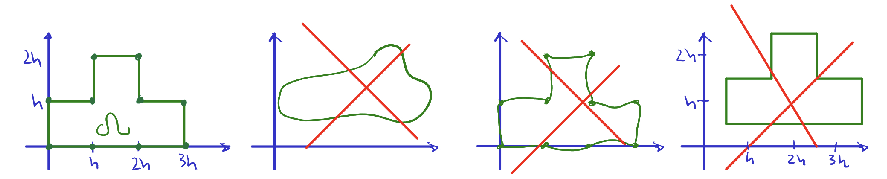
\includegraphics[width=14.8909550045914cm,height=3.00327954873409cm]{k2-3.pdf}}
  \]
  {\hspace{1.7em}}Nur die erste Menge ist ein W{\"u}rfelgebiet zu
  Wurfelseitenl{\"a}nge $h$, aber die vierte Menge ist ein W{\"u}rfelgebiet zu
  Wurfelseitenl{\"a}nge $\frac{h}{2}$. 
\end{example*}

Man sieht leicht, dass ein W{\"u}rfelgebiet zu $h \in \mathbb{R}_+$ auch ein
W{\"u}rfelgebiet zu $h / n$ f{\"u}r jedes $n \in \mathbb{N}$ ist.

\begin{definition}
  \tmtextbf{(FD-Gitter f{\"u}r W{\"u}rfelgebiet)}
  
  \tmtextit{Sei $\Omega \subseteq \mathbb{R}^d$ ein W{\"u}rfelgebiet zu $h \in
  \mathbb{R}^d$, $\Gamma \assign \partial \Omega$ also $\bar{\Omega} \assign
  \Omega \cup \Gamma$.
  
  Wir definieren das {\underline{Gitter}} $\bar{\Omega}_h$ durch
  \begin{eqnarray*}
    \Omega_h & \assign & \{ x \in \Omega | \nobracket \exists z \in
    \mathbb{Z}^d : x = h z \}\\
    \Gamma_h & \assign & \{ x \in \Gamma | \nobracket \exists z \in
    \mathbb{Z}^d : x = h z \}\\
    \bar{\Omega}_h & \assign & \Omega_h \cup \Gamma_h .
  \end{eqnarray*}}
\end{definition}

\begin{remark*}
  {\tmdummy}
  
  \begin{itemizedot}
    \item Jeder Punkt in $\Omega_h$ hat genau $2 d$ direkte Nachbaren mit
    Abstand $h$ in $\bar{\Omega}_h$.
    
    \item Erweiterung f{\"u}r allgemeine Gebiete folgt sp{\"a}ter. 
  \end{itemizedot}
\end{remark*}

\begin{definition}
  \tmtextbf{(Gitterfunktion)}
  
  \tmtextit{Zu einem Gitter $\bar{\Omega}_h$ definieren wir den
  {\underline{Raum der Gitterfunktionen}}
  \[ X_h \assign \{ v : \bar{\Omega}_h \rightarrow \mathbb{R} \}, \]
  davon den {\underline{Teilraum der Funktionen mit Nullrandwerten}}
  \[ X^{\circ}_h \assign \{ v \in X_h  | \nobracket \forall x \in \Gamma_h : v
     (x) = 0 \} \subseteq X_h, \]
  und au{\ss}erdem den {\underline{Raum der Funktionen der inneren Punkte}}
  \[ Y_h \assign \{ v : \Omega_h \rightarrow \mathbb{R} \} \]
  jeweils versehen mit Maximumsnormen
  \[ \| v \|_{\bar{\Omega}_h} \assign \max_{x \in \bar{\Omega}_h} | v (x) |
     \text{\qquad bzw.\qquad} \| v \|_{\Omega_h} \assign \max_{x \in \Omega_h}
     | v (x) | . \]}
\end{definition}

\begin{remark*}
  \tmtextbf{(Zus{\"a}tzliche Raumstruktur)}
  \begin{itemizedot}
    \item $(X_h, \| \bullet \|_{\bar{\Omega}_h})$, $(X^{\circ}_h, \| \bullet
    \|_{\bar{\Omega}_h})$, $(X_h, \| \bullet \|_{\Omega_h})$ sowie $(Y_h, \|
    \bullet \|_{\Omega_h})$ sind Banachr{\"a}ume, da endlich dimensional und
    damit vollst{\"a}ndig.
    
    \item Man kann $X_h$ auch mit einer Hilbertraumstruktur versehen, indem
    man das ,,diskrete $l^2$-Skalarprodukt`` definiert, also
    \[ \langle u, v \rangle_{l^2} \assign h^d \sum_{x \in \bar{\Omega}_h} u
       (x) v (x) \]
    welches die Norm $\| u \|_{l^2} \assign \sqrt{\langle u, u \rangle_{l^2}}
    = \sqrt{h^d \sum_{x \in \bar{\Omega}_h} u (x) u (x)}$ induziert.
    
    \item Bzgl. $\| \bullet \|_{l^2}$ ist $X_h$ ebenfalls vollst{\"a}ndig,
    und es gilt sogar
    \[ \forall u \in C^0 (\bar{\Omega}) : \text{\quad} \lim_{h \rightarrow 0}
       \| u \|_{l^2} = \| u \|_{L^2} . \]
    \item Man kann $X_h$ auch mit einer Seminorm versehen, welche die
    Ableitungen mit einbezieht (,,diskrete $H^1$-Seminorm``)
    \[ | u |_{h^1} \assign \sqrt{h^d \sum_{x \in \Omega_h} \sum_{j = 1}^d
       (\partial_{x_j}^{+ h} u (x))^2} . \]
    Dies ist nur eine Seminorm auf $X_h$ aber eine Norm auf $X_h^0$. Damit
    erh{\"a}lt durch Kombination mit $l^2$-Norm eine Norm auf $X_h$
    (,,diskrete $H^1$-Norm``)
    \[ \| u \|_{h^1} \assign \sqrt{\| u \|_{l^2}^2 + | u |_{h^1}^2} \]
    bzgl. welcher $X_h$ auch Hilbertraum ist. Details dazu kommen im Kapitel
    3.
  \end{itemizedot}
\end{remark*}

Wir bemerken hier noch: F{\"u}r $v \in X_h$ und $x \in \Omega_h$ ist mit (2.6)
$(- \nonconverted{bigtriangleup}_h v) (x)$ wohldefiniert, d.h. wir k{\"o}nnen
$\nonconverted{bigtriangleup}_h : X_h \rightarrow Y_h$ als linearen Operator
interpretieren.

\begin{definition}
  \tmtextbf{(FD-Approximation f{\"u}r Poisson-RWP)}
  
  \tmtextit{Sei ein Gitter $\bar{\Omega}_h$ gegeben.
  
  Dann nennen wir $u_h \in X_h$ eine {\underline{FD-Approximation des
  Poisson-RWP}} aus Korrolar 2.28, g.d.w. es gilt
  \begin{equation}
    \begin{array}{lllll}
      \forall x \in \Omega_h : &  & - \Delta_h u_h (x) & = & f (x),\\
      \forall x \in \Gamma_h : &  & u_h (x) & = & g (x) .
    \end{array}
  \end{equation}}
\end{definition}

\begin{remark*}
  \tmtextbf{(Berechnung via LGS)}
  \begin{itemizedot}
    \item Sei eine Aufz{\"a}hlung $\{ x_1, \ldots, x_n \} = \Omega_h$ gegeben.
    Dann ist (2.7) {\"a}quivalent zu LGS f{\"u}r unbekannte $\vec{u}_h \assign
    \{ u_i \}_{i = 1}^n$ mit $u_i \assign u_h (x_i)$ f{\"u}r $i \in \{ 1,
    \ldots, n \}$, denn f{\"u}r $x \in \Gamma_h$ ist $u_h (x)$ schon durch $g
    (x)$ festgelegt.
    
    \item Sei FD-Operator in $x_i \in \Omega_h$ gegeben durch
    \[ - \Delta_h u_h (x_i) = \sum_{j = 1}^n \alpha_{i j} u (x_j) + \sum_{x
       \in \Gamma_h} \beta_{i, x} u (x) \]
    wobei $\sum_{j = 1}^n \alpha_{i j} u (x_j)$ den Anteil f{\"u}r die Punkte
    in $\Omega_h$ ist und $\sum_{x \in \Gamma_h} \beta_{i, x} u (x)$ f{\"u}r
    den Rand.
    
    Dann ist ein LGS gegeben durch
    \[ A_h  \vec{u}_h = b_h \]
    mit $A_h = (\alpha_{i j})_{i, j = 1}^n$ und $b_h = \left( f (x_i) -
    \sum_{x \in \Gamma_h} \beta_{i, x} u (x) \right)_{i = 1}^n$.
    
    \item Beachte: $A_h$ ist d{\"u}nn besetzt (sparse), da es nur sehr wenige
    Nichtnull-Eintr{\"a}ge pro Zeile gibt, daher in Praxis
    Sparse-Matrix-Datenstruktur verwendet wird. 
  \end{itemizedot}
\end{remark*}

\begin{example}
  \tmtextbf{(FD-Approximation f{\"u}r Poisson-RWP in 1D)}
  
  Sei $d \assign 1$, $\Omega \assign (0, 1)$, $n \in \mathbb{N}$, $h \assign
  \frac{1}{n + 1}$, $x_i \assign i h$ f{\"u}r $i \in \{ 0, \ldots, n + 1 \}$,
  dann ist
  \[ \Omega_h \assign \{ x_1, \ldots, x_n \}, \text{\qquad} \Gamma_h \assign
     \{ x_0, x_{n + 1} \} . \]
  {\hspace{1.7em}}Poisson-Problem:
  \[ \begin{array}{l}
       - u'' (x) = f (x) \quad \text{in } \Omega,\\
       u (0) = \alpha, \text{\quad} u (1) = \beta .
     \end{array} \]
  {\hspace{1.7em}}Sei $u_i \approx u (x_i)$ f{\"u}r $i \in \{ 1, \ldots, n
  \}$, $u_0 \assign \alpha$ und $u_{n + 1} \assign \beta$.
  
  Zugeh{\"o}rige Diskretisierung
  \[ \forall i \in \{ 1, \ldots, n \} : \text{\qquad} - \frac{u_{i + 1} - 2
     u_i + u_{i - 1}}{h^2} = f (x_i) \]
  und somit LGS
  \[ \begin{array}{llll}
       \text{\qquad} \tilde{A}_n &  &  & \\
       \underbrace{\frac{1}{h^2} \overbrace{\left(\begin{array}{cccc}
         2 & - 1 &  & \\
         - 1 & 2 & \ddots & \\
         & \ddots & \ddots & - 1\\
         &  & - 1 & 2
       \end{array}\right)}} & \underbrace{\left(\begin{array}{c}
         u_1\\
         \vdots\\
         u_n
       \end{array}\right)} & = & \underbrace{\left(\begin{array}{c}
         f (x_1) + \frac{\alpha}{h^2}\\
         f (x_2)\\
         \vdots\\
         f (x_{n - 1})\\
         f (x_n) + \frac{\beta}{h^2}
       \end{array}\right)}\\
       \text{\enspace} A_h & \vec{u}_h &  & \text{\enspace} b_h .
     \end{array} \]
\end{example}

\begin{remark*}
  {\tmdummy}
  
  \begin{itemizedot}
    \item $\tilde{A}_n$ und $A_h$ sind tridiagonal und symmetrisch und klar
    ist $A_h \assign \frac{1}{h^2} \tilde{A}_n$.
    
    \item $A_h$ ist regul{\"a}r, denn per Induktion folgt $\det \tilde{A}_n =
    n + 1$:
    
    F{\"u}r $n = 1$ ist $\det (\tilde{A}_n) = \det (2) = n + 1$.
    
    Im Induktionsschritt $n \rightarrow n + 1$ gilt mit Laplace-Entwicklung:
    \begin{eqnarray*}
      \det (\tilde{A}_{n + 1}) & = & \det \left(\begin{array}{cc}
        \tilde{A}_n & \begin{array}{c}
          0\\
          \vdots\\
          0\\
          - 1
        \end{array}\\
        \begin{array}{l}
          0 \cdots 0 \enspace - 1
        \end{array} & 2
      \end{array}\right)\\
      & = & 2 \det (\tilde{A}_n) - (- 1) \det \left(\begin{array}{cc}
        \tilde{A}_{n - 1} & \begin{array}{c}
          0\\
          \vdots\\
          0
        \end{array}\\
        \begin{array}{l}
          0 \cdots 0 \enspace - 1
        \end{array} & - 1
      \end{array}\right)\\
      & = & 2 \det (\tilde{A}_n) + (- 1) \det (\tilde{A}_{n - 1})\\
      & = & 2 \hspace{1.3em} n \hspace{1.4em} + (- 1) \quad (n - 1) .
    \end{eqnarray*}
    \item $A_h$ ist positiv definit, denn mit Satz von Gerschgorin ist
    $\lambda_i (A_h) \in [0, 4]$ und wegen Regularit{\"a}t von $A_h$ ist sogar
    $\lambda_i (A_h) \in (0, 4]$.
    
    \item Damit existiert eindeutige FD-Approximation $u_h$ des Poisson-RWP in
    1D.
    
    \item Wegen $A_h$ positiv definit \& symmetrisch kann CG oder PCG als
    iterative LGS-L{\"o}ser verwendet werden.
    
    \item F{\"u}r kleine $h$ ist $A_h$ und $\tilde{A}_n$ schlecht
    konditioniert, also ist Vorkonditionierung zu empfehlen.
    
    \item Man kann f{\"u}r das diskrete Problem auch ,,stetige
    Abh{\"a}ngigkeit von den Daten`` beweisen (siehe {\"U}bung). 
  \end{itemizedot}
\end{remark*}

\begin{example}
  \tmtextbf{(FD-Approximation f{\"u}r Poisson-RWP in 2D)}
  
  Sei $d \assign 2$, $\Omega \assign (0, 1)^2$, $m \in \mathbb{N}$, $h \assign
  \frac{1}{m + 1}$, $n \assign m^2$ und ein Poisson-RWP mit $g = 0$ gegeben.
  
  Statt Einzelindex nutzen wir zur besseren {\"U}bersicht Doppelindex, also:
  \[ \forall i, j \in \{ 0, \ldots, m + 1 \} : \text{\qquad} x_{i j} \assign
     (i h, j h), \text{\quad} u_{i, j} \approx u (x_{i j}) . \]
  {\hspace{1.7em}}Diekretisierung des RWP f{\"u}r $\forall i, j \in \{ 0,
  \ldots, m + 1 \}$:
  \begin{eqnarray*}
    \text{{\hspace{4em}}} & \frac{1}{h^2} (4 u_{i, j} - u_{i - 1, j} - u_{i +
    1, j} - u_{i, j - 1} - u_{i, j + 1}) = f (i h, j h) & \text{f{\"u}r innere
    Punkte,}\\
    & u_{0, j} = u_{m + 1, j} = u_{i, 0} = u_{i, m + 1} = 0 & \text{f{\"u}r
    Randpunkte} .
  \end{eqnarray*}
  {\hspace{1.7em}}F{\"u}r jede beliebige Wahl von Aufz{\"a}hlung der $u_{i,
  j}$ erh{\"a}lt man unter Anpassung der Umordnung ein System von LGS
  \[ A_h  \vec{u}_h = b_h \]
  wobei $A_h$ symmetrisch ist und $\frac{4}{h^2}$ auf Diagonalen sowie $-
  \frac{1}{h^2}$ an bis zu $4$ Stellen pro Zeilen und pro Spalte.
  
  Mit lexikographischer Aufz{\"a}hlung, also $\vec{u}_h = (u_{11}, u_{12},
  \ldots, u_{1 m}, u_{21}, \ldots, u_{m m})$, bekommt $A_h$ eine
  ,,Bandstruktur``, also ,,block-tridiagonal``, d.h.
  \[ A_h = \frac{1}{h^2} \left(\begin{array}{cccc}
       B & C &  & \\
       C & B & \ddots & \\
       & \ddots & \ddots & C\\
       &  & C & B
     \end{array}\right) \in \mathbb{R}^{m^2 \times m^2} \]
  wobei
  \[ \text{} B = \left(\begin{array}{cccc}
       4 & - 1 &  & \\
       - 1 & 4 & \ddots & \\
       & \ddots & \ddots & - 1\\
       &  & - 1 & 4
     \end{array}\right) \in \mathbb{R}^{m \times m}, \text{\quad} C = - I_m =
     \left(\begin{array}{ccc}
       - 1 &  & 0\\
       & \ddots & \\
       0 &  & - 1
     \end{array}\right) \in \mathbb{R}^{m \times m} . \]
\end{example}

\begin{remark*}
  \tmtextbf{(Erweiterung auf beliebige Gebiete)}
  \begin{itemizedot}
    \item Falls $\Omega$ beschr{\"a}nkt aber kein W{\"u}rfelgebiet ist, muss
    das Gitter modifiziert werden, indem Schnittpunkte von $\Gamma$ mit den
    von $\mathbb{Z}^d \cdot h$ erzeugten W{\"u}rfelkanten hinzugenommen
    werden:
    \[ \Gamma_h \assign \{ x \in \Gamma | \nobracket \exists j \in \{ 1,
       \ldots, d \} \exists z \in \mathbb{Z}^d : x \in h (z + \mathbb{R} e_j)
       \} \]
    dann wie gehabt $\bar{\Omega}_h \assign \Omega_h \cup \Gamma_h$ mit
    $\Omega_h$ aus Def. 2.36.
    \[ 
       \raisebox{-0.00268145657559141\height}{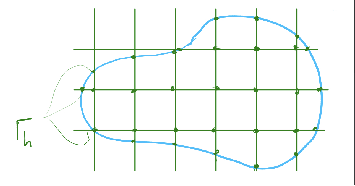
\includegraphics[width=5.96645021645022cm,height=3.13100157418339cm]{k2-4.pdf}}
    \]
    \item Koeffizienten der FD-Diskretisierung werden angepasst.
    \[ 
       \raisebox{-0.00246236714278844\height}{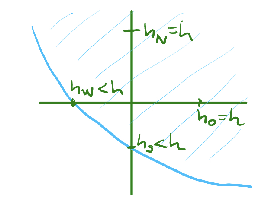
\includegraphics[width=4.47904368358914cm,height=3.40958284140102cm]{k2-5.pdf}}
    \]
    Taylor-Entwicklung liefert:
    
    1D:
    \begin{eqnarray*}
      u'' (x) & = & \frac{2}{h_W (h_O + h_W)} u (x - h_W) - \frac{2}{h_W h_O}
      u (x)\\
      &  & + \frac{2}{h_O (h_O + h_W)} u (x + h_O) + \mathcal{O} (h) .
    \end{eqnarray*}
    {\hspace{1.7em}}2D:
    \begin{eqnarray*}
      \Delta u (x) & = & \frac{2}{h_W (h_O + h_W)} u (x - e_1 h_W) +
      \frac{2}{h_O (h_O + h_W)} u (x + e_1 h_O)\\
      &  & + \frac{2}{h_S (h_S + h_N)} u (x - e_2 h_S) + \frac{2}{h_N (h_S +
      h_N)} u (x + e_2 h_N)\\
      &  & - \left( \frac{2}{h_O h_W} + \frac{2}{h_S h_N} \right) u (x) +
      \mathcal{O} (h) .
    \end{eqnarray*}
    Dies ist die {\underline{\tmtextit{Shortly-Weller-Approximation}}}.
    
    \item Man verliert also eine $h$-Potenz in der Approximationsg{\"u}te.
    
    \item Systemmatrix wird i.A. nicht symmetrisch. 
  \end{itemizedot}
\end{remark*}

\begin{remark*}
  \tmtextbf{(Andere Randbedingungen)}
  
  Neben Dirichlet auch andere Randbedingungen m{\"o}glich, z.B.
  Neumann-Randbedingung:
  \[ \forall x \in \Gamma_N \subseteq \Gamma \text{wobei } \Gamma_N 
     \text{Neumann-Randteil:} \quad (\nabla u (x)) \bullet n = g_N (x) . \]
  {\hspace{1.7em}}Wir nehmen zus{\"a}tzlich an, dass $x$ auf Kante und nicht
  auf Ecke des W{\"u}rfelgebiets liegt, sonst ist keine Normale $n (x)$
  definiert.
  \[ \tmop{Hier} \tmop{fehlt} \tmop{eine} \tmop{Skizze} \ldots . \]
  Sei $n = \pm e_j$ {\"a}u{\ss}erer Normalenvektor f{\"u}r ein $j \in \{ 1,
  \ldots, d \}$.
  
  Wir approximieren $\nabla u$ durch
  \[ (\nabla_h u)_i \assign \left\{\begin{array}{ll}
       \partial_{x_i}^{c, h} u & \text{ f{\"u}r } i \neq j \text{(zentrale
       Diff.)}\\
       \partial_{x_j}^{- h} u & \text{ f{\"u}r } i = j
       \text{(R{\"u}ckw{\"a}rts-Diff.)}
     \end{array}\right. \]
  {\hspace{1.7em}}F{\"u}r $x \in \Gamma_h \cap \Gamma_N$ ist nun $u_h (x)$
  auch Unbekannte, denn man kennt nicht seinen Funktionswert, nur die
  Ableitung.
  
  Also neue Gleichung f{\"u}r LGS:
  \[ \forall x \in \Gamma_h \cap \Gamma_N : \text{\quad} (\nabla_h u_h (x))
     \bullet n = g_N (x) . \]
\end{remark*}

\

\section{FD f{\"u}r allgemeine elliptische PDEs 2. Ordnung}

\begin{definition}
  \tmtextbf{(Allgemeine Elliptisches RWP)}
  
  \tmtextit{Zu einem beschr{\"a}nkten Gebiet $\Omega \subseteq \mathbb{R}^d$,
  einer $f \in C^0 (\Omega)$ und einer $g \in C^0 (\Omega)$ sei
  \begin{equation}
    (\mathscr{L} u) (x) = - \sum_{i, j = 1}^d a_{i j} (x) \partial_{x_i}
    \partial_{x_j} u (x) + \sum_{i = 1}^d b_i (x) \partial_{x_i} u (x) + c (x)
    u (x)
  \end{equation}
  gleichm{\"a}{\ss}ig elliptisch und $a_{i j}$, $b_i$, $c \in C^0
  (\bar{\Omega})$.
  
  Gesucht ist $u \in C^2 (\Omega) \cap C^0 (\bar{\Omega})$ mit den
  Eigenschaften
  \begin{eqnarray*}
    (\mathcal{\mathscr{L}} u) (x) = f (x) &  & \text{f{\"u}r } x \in \Omega,\\
    u (x) = g (x) &  & \text{f{\"u}r } x \in \Gamma .
  \end{eqnarray*}}
\end{definition}

\begin{definition}
  \tmtextbf{(FD-Approximation)}
  
  F{\"u}r $\mathcal{\mathscr{L}}$ aus (2.8), $u \in C^2 (\Omega) \cap C^0
  (\bar{\Omega})$, $h \in \mathbb{R}_+$, $x \in \Omega$ mit $\overline{B_h
  (x)} \subseteq \bar{\Omega}$ definieren wir
  \begin{eqnarray*}
    (\mathcal{\mathscr{L}}_h u) (x) & \assign & - \sum_{i = 1}^d a_{i i} (x)
    \partial^{- h}_{x_i} \partial^{+ h}_{x_i} u (x) - \sum_{i, j = 1}^d a_{i
    j} (x) \partial^{c, h}_{x_i} \partial^{c, h}_{x_j} u (x)\\
    &  & + \sum_{i = 1}^d b_i (x) \partial^{c, h}_{ x_i} u (x) + c (x) u (x)
    .
  \end{eqnarray*}
\end{definition}

\begin{remark*}
  Wir werden sehen, dass
  \begin{itemizedot}
    \item Def. 2.42 nur unter zus{\"a}tzlichen Annahmen an $a_{i j}$, $b_i$,
    $c$, $h$ eine ,,stabile`` Diskretisierung ergibt;
    
    \item eine etwas sorgf{\"a}ltigere Diskretisierung des Hauptteils eine
    erweiterte Klasse von Funktionen $a_{i j}$, $b_i$, $c$ ,,stabil``
    diskretisiert.
  \end{itemizedot}
\end{remark*}

\begin{theorem}
  \tmtextbf{(FD-Approximationsfehler f{\"u}r $\mathscr{L}_h$)}
  
  \tmtextit{Sei $u \in C^4 (\Omega)$}, $x \in \Omega$ \tmtextit{s.d. f{\"u}r
  $i \in \{ 1, \ldots, d \}$ und $\sigma_i \in \{ 0, 1, - 1 \}$ gilt} $x +
  \sum_{i = 1}^d \sigma_i e_i h$.
  
  \tmtextit{Dann existiert ein $C$} \tmtextit{(unabh{\"a}ngig von $x$ und
  $h$), s.d. }
  \[ | (\mathcal{\mathscr{L}} u) (x) - (\mathcal{\mathscr{L}}_h u) (x) | \leq
     C \cdot h^2 . \]
\end{theorem}

\begin{proof}
  Mittels Taylor, analog zu 2.33 \& 2.34. 
\end{proof}

\begin{remark*}
  \tmtextbf{(FD-Stern)}
  \begin{itemizedot}
    \item Die Diskretisierung eines PDE-Operators $\mathscr{L}$ kann man
    anschaulicher notieren, z.B. f{\"u}r $d = 2$ und um $(x_1, x_2)$ herum:
    
    Falls $(\mathcal{\mathscr{L}}_h u) (x_1, x_2) = \frac{1}{h^2} \sum_{i, j =
    - m}^m \alpha_{i j} u (x_1 + i h, x_2 + j h)$ f{\"u}r ein $m \in
    \mathbb{N}$ und geeignete Koeffizieten $\alpha_{i j}$, so ist
    \begin{equation}
      \left(\begin{array}{ccccc}
        \alpha_{- m, m} & \cdots & \alpha_{0, m} & \cdots & \alpha_{m, m}\\
        \vdots &  & \vdots &  & \vdots\\
        \alpha_{- m, 0} & \cdots & \alpha_{0, 0} & \cdots & \alpha_{m, 0}\\
        \vdots &  & \vdots &  & \vdots\\
        \alpha_{- m, - m} & \cdots & \alpha_{0, - m} & \cdots & \alpha_{m, -
        m}
      \end{array}\right)_{\ast}
    \end{equation}
    der zugeh{\"o}rige FD-Stern.
    
    \item F{\"u}r $\mathcal{\mathscr{L}}_h u = -
    \nonconverted{bigtriangleup}_h$ aus Fol. 2.34 ergibt sich also f{\"u}r $m
    = 1$
    \[ \left(\begin{array}{ccc}
         0 & - 1 & 0\\
         - 1 & 4 & - 1\\
         0 & - 1 & 0
       \end{array}\right)_{\ast} \]
    der 5-Punkte-Differenzen-Stern.
    
    \item F{\"u}r $\mathscr{L}_h$ aus Def. 2.42 ergibt sich der FD-Stern als
    (oBdA $a_{12} = a_{21}$)
    \begin{equation}
      \begin{array}{l}
        \frac{1}{2} \left(\begin{array}{ccc}
          a_{12} (x) & - 2 a_{22} (x) & - a_{12} (x)\\
          - 2 a_{11} (x) & 4 (a_{11} (x) + a_{22} (x)) & - 2 a_{11} (x)\\
          - a_{12} (x) & - 2 a_{22} (x) & a_{12} (x)
        \end{array}\right)_{\ast}\\
        + \frac{h}{2} \left(\begin{array}{ccc}
          0 & b_2 (x) & 0\\
          - b_1 (x) & 0 & b_1 (x)\\
          0 & - b_2 (x) & 0
        \end{array}\right)_{\ast} + h^2 \left(\begin{array}{ccc}
          0 & 0 & 0\\
          0 & c (x) & 0\\
          0 & 0 & 0
        \end{array}\right)_{\ast}
      \end{array}
    \end{equation}
    \item F{\"u}r $m = 1$ (also $3 \times 3$ Sterne) ist h{\"o}chstens
    Approximationsordnung 2 erreichbar, wie in 2.43 \& 2.34 f{\"u}r spezielle
    $\mathcal{\mathscr{L}}_h$ realisiert.
    
    \item F{\"u}r $m > 1$ sind bessere Approximationsordnung erreichbar. 
  \end{itemizedot}
\end{remark*}

\begin{definition}
  \tmtextbf{(FD-Approximation f{\"u}r elliptisches RWP)}
  
  \tmtextit{Sei $\Omega$ W{\"u}rfelgebiet zu $h \in \mathbb{R}_+$ und
  $\bar{\Omega}_h$ das zugeh{\"o}rige Gitter.
  
  Dann ist $u_h \in X_h$ {\underline{FD-Approximation des elliptischen RWP}},
  g.d.w. es gilt
  \begin{eqnarray*}
    (\mathcal{\mathscr{L}}_h u_h) (x) = f (x) &  & \text{f{\"u}r } x \in
    \Omega_h,\\
    u_h (x) = g (x) &  & \text{f{\"u}r } x \in \Gamma_h .
  \end{eqnarray*}}
\end{definition}

\begin{definition}
  \tmtextbf{(Diskreter Zusammenhang)}
  
  \tmtextit{Ein Gitter $\bar{\Omega}_h$ hei{\ss}t {\underline{diskrete
  zusammenh{\"a}ngend}}, g.d.w. es f{\"u}r alle $x$, $y \in \Omega_h$ (also
  innere Punkte) eine Punktfolge $z_1, \ldots, z_k \in \Omega_h$ s.d.
  \[ z_0 = x, \text{\quad} z_k = y, \text{\quad} | z_2 - z_1 | = \cdots = |
     z_k - z_{k - 1} | = h. \]}
\end{definition}

\begin{example*}
  \
  
  Falls $\Omega$ zusammenh{\"a}ngend, ist f{\"u}r gen{\"u}gend kleines $h$
  auch $\bar{\Omega}_h$ diskret zusammenh{\"a}ngend, z.B.
  \[ 
     \raisebox{-0.00229643783022507\height}{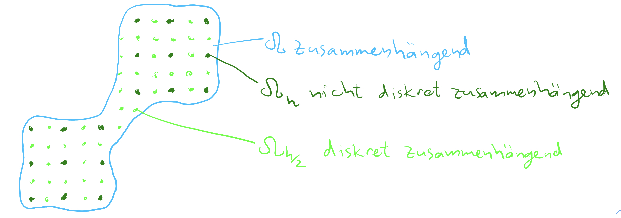
\includegraphics[width=10.4287026105208cm,height=3.65594254230618cm]{k2-6.pdf}}
  \]
\end{example*}

Bei der Untersuchung von FD-Stern hilft uns folgendes technisches Lemma:

\begin{lemma}
  \tmtextbf{(Sternlemma)}
  
  \tmtextit{Sei $k \in \mathbb{N} $, $\{ \alpha_i \}_{i = 0}^k \subseteq
  \mathbb{R}$ und $\{ p_i \}_{i = 0}^k \subseteq \mathbb{R}$ gegeben s.d.
  \[ \alpha_0 > 0, \text{\quad} \alpha_1, \ldots, \alpha_k < 0, \text{\quad}
     \sum_{i = 0}^k \alpha_i = 0, \text{\quad} \sum_{i = 0}^k \alpha_i p_i
     \leqslant 0, \text{\quad} p_0 = \max_{i \in \{ 1, \ldots, k \}} p_i . \]
  {\hspace{1.7em}}Dann folgt $p_0 = p_1 = \cdots = p_k$.}
\end{lemma}

Bei Anwendung des Lemma sp{\"a}ter werden die $\alpha_i$ die FD-Koeffizienten
sein, und $p_i$ die L{\"o}sungswerte in den Punkten. Das Lemma dient mehr oder
weniger als ein Kriterium f{\"u}r die Konstantheit der L{\"o}sungswerten. \

\begin{proof}
  \
  
  Mit $\text{} p_0 = \max_{i \in \{ 1, \ldots, k \}} p_i$ und $\alpha_1,
  \ldots, \alpha_k < 0$ ist $\alpha_i (p_i - p_0) \geq 0$ f{\"u}r jedes $i \in
  \{ 1, \ldots, k \}$, und somit
  \begin{eqnarray*}
    0 \leqslant \sum_{i = 0}^k \alpha_i (p_i - p_0) & = & \underbrace{\sum_{i
    = 0}^k \alpha_i p_i} - p_0 \underbrace{\sum_{i = 0}^k \alpha_i} \leqslant
    0\\
    &  & \text{{\hspace{1.5em}}} \leqslant 0 \hspace{3.5em} = 0
  \end{eqnarray*}
  also ist $\sum_{i = 0}^k \alpha_i (p_i - p_0) = 0$, und da alle $\alpha_i$
  von $0$ verschieden sind, m{\"u}ssen alle $p_i$ gleich sind. 
\end{proof}

Mit diesem Lemma kann f{\"u}r gewisse $\mathscr{L}_h$ ein diskretes Analogon
des Maximumsprinzips 2.27 gezeigt werden.

Dies impliziert dann analoge Aussagen wie im Kontinuierlichen.

\begin{theorem}
  \tmtextbf{(Diskretes Maximumsprinzip)}
  
  \tmtextit{Sei $u_h \in X_h$ FD-Approximation des RWP 2.44 mit $f (x)
  \leqslant 0$ f{\"u}r $\forall x \in \Omega_h$.
  
  Der Differenzenstern (2.9) zu $m = 1$ (also $3 \times 3$ Stern) erf{\"u}lle
  in allen Punkten
  
  
  \[ \begin{array}{ll}
       \text{i.} & \sum_{i, j = - 1}^1 \alpha_{i j} = 0
     \end{array} \hspace{3em} \begin{array}{ll}
       \text{iii.} & \forall (i, j) \neq (0, 0) : \alpha_{i j} \leqslant 0
       \hspace{7em}
     \end{array} \]
  \[ \begin{array}{ll}
       \text{ii.} & \alpha_{00} > 0 \qquad
     \end{array} \hspace{3.5em} \begin{array}{ll}
       \text{iv.} & \alpha_{1, 0} < 0, \text{\enspace$\alpha_{0, 1} < 0,
       \text{\enspace} \alpha_{- 1, 0} < 0, \text{\enspace} \alpha_{0, - 1} <
       0$} .
     \end{array} \]
  {\hspace{1.7em}}Dann gilt
  \[ \max_{x \in \overline{\Omega }_h} u_h (x) = \max_{x \in \Gamma_h} u_h
     (x) . \]}
\end{theorem}

\begin{proof}
  Sei $x \in \overline{\Omega }_h$ mit $u_h (x) = \max_{x \in \Gamma_h} u_h
  (x)$.
  
  Falls $x \in \Gamma_h$, ist die Behauptung klar.
  
  Falls $x \in \Omega_h$, setze $p_0 \assign u_h (x)$, $(p_i)_{i = 1}^k$ als
  Nachbarwerte von $u_h (x)$ und $\alpha_0 \assign \alpha_{00}$ und
  $(\alpha_i)_{i = 1}^k$ als Nicht-Null-Koeffizienten des FD-Sterns.
  
  Es gilt dann
  \[ \sum_{i = 0}^k \alpha_i p_i = (\mathcal{\mathscr{L}}_h u_h) (x) = f (x)
     \leqslant 0 \]
  also liefert das Sternlemma: $p_0 = p_1 = \cdots = p_k$, d.h. $u_h$ ist
  konstant auf $x$ und seinen Nachbarn, welche im Differenzenstern auftreten.
  \
  
  Wiederholung dieses Argumentes in alle $2 d$ Hauptrichtungen f{\"u}hrt zum
  Rand wegen Beschr{\"a}nktkeit von $\Omega$.
\end{proof}

Falls $\bar{\Omega}_h$ diskret zusammenh{\"a}ngend ist, f{\"u}hrt das letzte
Argument zu allen Punkten in $\Omega_h$, also folgt:

\begin{corollary}
  \tmtextbf{(FD-Approximation $u_h$ konstant)}
  
  \tmtextit{Es gelten die Voraussetzungen von 2.47.
  
  Falls $\bar{\Omega}_h$ diskret zusammenh{\"a}ngend ist und FD-Approximation
  $u_h$ ihr Maximum im Inneren annimmt, so ist $u_h$ konstant. }
\end{corollary}

\begin{remark*}
  {\tmdummy}
  
  \begin{itemizedot}
    \item Obiges diskretes Maximumsprinzip gilt f{\"u}r $\mathscr{L}_h = -
    \Delta_h$, weil Voraussetzungen erf{\"u}llt sind.
    
    \item F{\"u}r $\mathscr{L}_h$ aus (2.10) mit $a_{12} = 0$, $c = 0$, $b
    \neq 0$ sind Voraussetzungen von 2.47 f{\"u}r ,,gen{\"u}gend kleines`` $h$
    erf{\"u}llt:
    
    Man nutzt die gleichm{\"a}{\ss}ige Elliptizit{\"a}t aus und erhl{\"a}t mit
    $z = e_i$ \
    \[ 0 < \alpha \leqslant \langle z, A (x) z \rangle = a_{i i} (x) \]
    also $\alpha_{00} = 2 a_{11} + 2 a_{22} > 0$.
    
    Falls es ein $B$ gibt s.d. alle $| b_i | \leq B$ und $h \leqslant
    \frac{2}{B} \alpha$, dann gilt f{\"u}r $\alpha_{1, 0}$
    \[ \alpha_{1, 0} = - a_{11} + \frac{h}{2} b_1 < - \alpha + \frac{2}{B}
       \alpha \frac{1}{2} B = 0. \]
    {\hspace{1.7em}}Analog folgt $\alpha_{- 1, 0} < 0$, $\alpha_{0, - 1} < 0$
    und \ $\alpha_{0, 1} < 0$.
    
    $\sum_{i, j = - 1}^1 \alpha_{i j} = 0$ ist klar da $c = 0$.
    
    \item Falls $c (x) > 0$ in (2,5), so ist $\sum_{i, j = - 1}^1 \alpha_{i j}
    > 0$. F{\"u}r diesen Fall kann man Abschw{\"a}chungen des
    Sternlemmas/diskretes Maximumsprinzip beweisen.
    
    \item Falls $a_{1, 2} \neq 0$, so ist Modifikation der Diskretisierung
    notwendig. (Dies wird sp{\"a}ter betrachtet)
  \end{itemizedot}
\end{remark*}

\begin{corollary}
  \tmtextbf{(Diskretes Vergleichprinzip)}
  
  \tmtextit{Seien $u_h$, $v_h \in X_h$ und es gelte
  \[ \begin{array}{lllll}
       \mathscr{L}_h u_h & \leqslant & \mathscr{L}_h v_h &  &
       \text{in{\hspace{0.3em}}} \Omega_h\\
       u_h & \leqslant & v_h &  & \text{auf{\hspace{0.3em}}} \Gamma_h
     \end{array} \]
  und das diskrete Maximumsprinzip.
  
  Dann gilt
  \[ \begin{array}{rllll}
       u_h & \leqslant & v_h &  & \text{auf{\hspace{0.3em}}} \bar{\Omega}_h .
     \end{array} \]}
\end{corollary}

\begin{proof}
  \
  
  F{\"u}r $w_h \assign u_h - v_h$ gilt
  \[ \begin{array}{lll}
       \mathscr{L}_h w_h = \mathscr{L}_h u_h - \mathscr{L}_h v_h \leqslant 0 &
       & \text{in{\hspace{0.3em}}} \Omega_h\\
       w_h \leqslant 0 &  & \text{auf{\hspace{0.3em}}} \Gamma_h .
     \end{array} \]
  {\hspace{1.7em}}Aus disrektem Maximumsprinzip folgt
  \[ \max_{x \in \bar{\Omega}_h} w_h (x) = \max_{x \in \Gamma_h} w_h (x)
     \leqslant 0 \]
  also $u_h \leqslant v_h$ in $\bar{\Omega}_h$.
\end{proof}

\begin{corollary}
  \tmtextbf{(Existenz \& Eindeutigkeit der FD-Approx. f{\"u}r ellip. RWP)}
  
  \tmtextit{Sei ein diskretisiertes RWP gem{\"a}{\ss} 2.44 gegeben und es
  gelte das diskrete Maximumsprinzip.
  
  Dann existiert eine eindeutige FD-Approximation $u_h \in X_h$. }
\end{corollary}

\begin{proof}
  Zun{\"a}chst die Eindeutigkeit:
  
  Seien $u_h$, $\tilde{u}_h \in X_h$ zwei L{\"o}sungen gegeben.
  
  Setze $v \assign u_h - \tilde{u}_h$, dann ist
  \[ \begin{array}{ll}
       \mathscr{L}_h v = \mathscr{L}_h u_h - \mathscr{L}_h \tilde{u}_h = f
       |_{\Omega_h} \nobracket - f |_{\Omega_h} \nobracket = 0 & \text{in }
       \Omega_h\\
       v = u_h - \tilde{u}_h = g |_{\Gamma_h} \nobracket - g |_{\Gamma_h}
       \nobracket = 0 & \text{auf } \Gamma_h .
     \end{array} \]
  {\hspace{1.7em}}Das diskrete Maximumsprinzip liefert
  \[ \forall x \in \bar{\Omega}_h : \text{\quad} v (x) \leqslant \sup_{y \in
     \Gamma_h} v (y) = 0. \]
  {\hspace{1.7em}}Analoge Argumentation f{\"u}r $- v$ liefert:
  \[ \forall x \in \bar{\Omega}_h : \text{\quad} - v (x) \leqslant \sup_{y
     \in \Gamma_h} - v (y) = 0 \]
  also $v = 0$ auf $\bar{\Omega}_h$.
  
  {\hspace{4em}}Zur Existenz:
  
  FD-Diskretisierung f{\"u}hrt auf $n \times n$ System
  \[ A_h \underline{u} \text{}_h = b_h \]
  mit $\ker (A_h) = 0$ wegen Eindeutigkeit, also ist $A_h$ invertierbar und
  somit ist $\underline{u} \text{}_h \assign A_h^{- 1} b_h$ der eindeutiger
  Koeffizientenvektor f{\"u}r $u_h$.
\end{proof}

\begin{corollary}
  \tmtextbf{(Stetige Abh{\"a}ngigkeit von Randdaten)}
  
  \tmtextit{Seien $u_h$, $\tilde{u}_h \in X_h$ FD-Approximation zum RWP 2.44
  mit identischem $f$ aber unterschieldichen Randdaten $g$, $\tilde{g}$ und es
  gelte das diskrete Maximumsprinzip.
  
  Dann gilt
  \[ \| u - \tilde{u} \|_{\bar{\Omega}_h} = \| g - \tilde{g} \|_{\Gamma_h}
     \assign \sup_{x \in \Gamma_h} | g (x) - \tilde{g} (x) | . \]}
\end{corollary}

\begin{proof}
  \
  
  Setze $v \assign u_h - \tilde{u}_h$, dann ist $\mathscr{L}_h v = 0$ in
  $\Omega_h$.
  
  Mit dem diskreten Maximumsprinzip folgt f{\"u}r $\forall x \in
  \bar{\Omega}_h$
  \[ v \leqslant \max_{y \in \Gamma_h} v (y) \leqslant \max_{y \in \Gamma_h} |
     v (y) | = \max_{y \in \Gamma_h} | g (y) - \tilde{g} (y) | \]
  und analog f{\"u}r $- v (x)$, und damit folgt die Behauptung.
\end{proof}

\begin{remark*}
  {\tmdummy}
  
  \begin{itemizedot}
    \item Anschauliche Bedeutung: Leichte {\"A}nderung in Daten ergibt nur
    leichte {\"A}nderung in der L{\"o}sung.
    
    \item {\"A}hnlich kann man stetige Abh{\"a}ngigkeit von rechter Seite $f$
    formulieren. 
  \end{itemizedot}
\end{remark*}

\begin{definition}
  \tmtextbf{(Stabilit{\"a}t, Konsistenz, Konvergenz)}
  
  \tmtextit{Sei $u \in C^2 (\Omega) \cap C^0 (\bar{\Omega})$ L{\"o}sung des
  elliptischen RWP 2.41 und $u_h \in X_h$ die FD-Approximation aus 2.44.
  
  Das FD-Verfahren hei{\ss}t
  \begin{enumerateroman}
    \item {\underline{konsistent mit Ordnung $p$}}, wenn f{\"u}r ein $C_c \in
    \mathbb{R}$ (abh{\"a}ngig von $u$ aber unabh{\"a}ngig von $h$) gilt
    \[ \| \mathscr{L}_h u - \mathscr{L} u \|_{\Omega_h} \leqslant C_c h^p .
    \]
    \item {\underline{stabil}}, oder genauer {\underline{$(X_h^{\circ},
    Y_h)$-stabil}}, wenn f{\"u}r ein $C_s$ (abh{\"a}ngig von $u$ aber
    unabh{\"a}ngig von $h$) gilt
    \[ \forall v_h \in X_h^{\circ} : \text{\quad} \| v_h \|_{\bar{\Omega}_h}
       \leqslant C_s \| \mathscr{L}_h v_h \|_{\Omega_h} . \]
    \item {\underline{konvergent mit Ordnung $p$}}, wenn f{\"u}r ein $C$
    (abh{\"a}ngig von $u$ aber unabh{\"a}ngig von $h$) gilt
    \[ \| u - u_h \|_{\Omega_h} \leqslant C h^p . \]
  \end{enumerateroman}}
\end{definition}

\begin{remark*}
  \tmtextbf{(Konsistenz der FD-Approximation)}
  \begin{itemizedot}
    \item Punkweise Fehlerschranken aus 2.34 \& 2.43 besagten:
    \[ | \mathscr{L}_h u (x) - \mathscr{L} u (x) | \leqslant C h^2 \]
    mit $C$ unabh{\"a}ngig von $x$, also uniforme Schranke bzgl. $x$ falls $u
    \in C^4 (\Omega)$. Mit $C_c = C$ gilt also Konsistenz der FD-Approximation
    mit Ordnung $2$ falls $\Omega_h$ ein W{\"u}rfelgebiet ist.
    
    \item F{\"u}r $\Omega$ ein allgemeines Nicht-W{\"u}rfelgebiet ist i.A. die
    Konsistenzordnung der FD-Approximation geringer, z.B. von Ordnung $1$ bei
    Shortley-Weller-Approximation.
  \end{itemizedot}
\end{remark*}

\begin{remark*}
  \tmtextbf{(Stabilit{\"a}t)}
  
  Stabilit{\"a}t im Sinne von Def. 2.52 ii) bedeutet anschaulich, dass die
  FD-Approximation durch die rechte Seite unabh{\"a}ngig von $h$
  beschr{\"a}nkt bleibt:
  
  Sei $w_h : \Omega_h \rightarrow \mathbb{R}$ also $w_h \in Y_h$ und $v_h \in
  X^{\circ}_h$ L{\"o}sung von
  \[ \begin{array}{lllll}
       \mathscr{L}_h v_h & = & w_h &  & \text{in } \Omega_h\\
       v_h & = & 0 &  & \text{auf } \Gamma_h
     \end{array} \]
  dann ist also
  \[ \| v_h \|_{\bar{\Omega}_h} \leqslant C_s \| \mathscr{L}_h v_h \| = C_s
     \| w_h \|_{\Omega_h} . \]
\end{remark*}

\begin{theorem}
  \tmtextbf{(Hinreichende Bedingung f{\"u}r Stabilit{\"a}t)}
  
  \tmtextit{Sei $A_h \in \mathbb{R}^{n \times n}$ die FD-Systemmatrix.
  
  Falls es eine Konstante $C_s$ unabh{\"a}ngig von $h$ existiert, s.d.
  \[ \| A_h^{- 1} \|_{\infty} \leqslant C_s \]
  gilt, dann ist das FD-Verfahren stabil.}
\end{theorem}

\begin{proof}
  \
  
  Seien $\underline{v} \text{}_h$, $\underline{w} \text{}_h \in \mathbb{R}^n$
  Vektoren der inneren Knotenwerte f{\"u}r $v_h \in X_h^{\circ}$ sowie $w_h
  \in Y_h$, also $A_h \underline{v} \text{}_h = \underline{w} \text{}_h$, bzw.
  $\mathscr{L}_h v_h = w_h$.
  
  Dann erhalten wir
  \[ \| v_h \|_{\bar{\Omega}_h} = \left\| \underline{v} \text{}_h
     \right\|_{\infty} = \left\| A^{- 1}_h \underline{w} \text{}_h
     \right\|_{\infty} \leqslant \| A^{- 1}_h \|_{\infty} \left\|
     \underline{w} \text{}_h \right\|_{\infty} \leqslant C_s \| w_h
     \|_{\Omega_h} = C_s \| \mathscr{L}_h v_h \|_{\Omega_h} . \]
\end{proof}

\begin{theorem}
  \tmtextbf{(Stabilit{\"a}t f{\"u}r Poisson-RWP mit FD-Diskretisierung)}
  
  \tmtextit{Sei $\Omega \subseteq \mathbb{R}^d$ beschr{\"a}nktes Gebiet mit
  $\Omega \subseteq B_R (0)$ f{\"u}r ein $R \in \mathbb{R}_+$.
  
  Dann gilt f{\"u}r alle $v_h \in X_h^{\circ}$
  \[ \| v_h \|_{\bar{\Omega}_h} \leqslant \frac{R^2}{2 d} \|
     \nonconverted{bigtriangleup}_h v_h \|_{\Omega_h} \]
  also ist das FD-Verfahren stabil mit $C_s \assign \frac{R^2}{2 d}$.}
\end{theorem}

F{\"u}r den Beweis von 2.54 zeigen wir zun{\"a}chst eine Hilfsaussage:

\begin{lemma}
  \
  
  F{\"u}r $w_h \in X_h$ eine L{\"o}sung von
  \[ \begin{array}{lllll}
       - \Delta_h w_h & = & 1 &  & \text{in } \Omega_h\\
       w_h & = & 0 &  & \text{auf } \Gamma_h
     \end{array} \]
  gilt
  \begin{equation}
    \forall x \in \bar{\Omega}_h : \text{\quad} 0 \leqslant w_h (x) \leqslant
    \frac{1}{2 d} (R^2 - \| x \|^2_2) .
  \end{equation}
\end{lemma}

\begin{proof}
  \
  
  Sei $w (x) \assign \frac{1}{2 d} (R^2 - \| x \|^2_2)$, also kann man $w$
  als ein Produkt von mehreren Polynomen einer Variable sehen, und somit ist
  $\nonconverted{bigtriangleup}_h$ exakt f{\"u}r $w$ gem{\"a}{\ss} Kor. 2.34
  bzw. die Bemerkung danach.
  
  Daher gilt f{\"u}r jedes $x \in \Omega_h$
  \begin{eqnarray*}
    - \Delta_h w (x) & = & - \Delta w (x)\\
    & = & - \sum_{i = 1}^d \partial^2_{x_i} (R^2 - \| x \|^2_2) \frac{1}{2
    d}\\
    & = & - \sum_{i = 1}^d (- 2)  \frac{1}{2 d}\\
    & = & 1\\
    & = & - \Delta_h w_h (x) .
  \end{eqnarray*}
  {\hspace{1.7em}}Weiter ist $w \geqslant 0 = w_h$ auf $\Gamma_h$ nach Wahl
  von $R$.
  
  Aus dem diskreten Vergleichsprinzip 2.49 folgt $w \geq w_h$ auf
  $\bar{\Omega}_h$, also gilt die zweite Ungleichung in (2.11).
  
  Die erste Ungleichung in (2.11) folgt aus diskretem Maximumsprinzip f{\"u}r
  $- w_h$:
  \begin{eqnarray*}
    \forall x \in \Omega_h : \text{ } - \Delta_h (- w_h) = - 1 \leqslant 0 &
    \Rightarrow & \max_{x \in \bar{\Omega}_h} - w_h (x) \leqslant \max_{x \in
    \Gamma_h} - w_h (x) = 0\\
    & \Rightarrow & \forall x \in \bar{\Omega}_h : \text{ } w_h \geqslant 0.
  \end{eqnarray*}
  und damit sind wir fertig mit dem Nachweis der Hilfsaussage.
\end{proof}

\begin{proof}
  (von 2.54)
  
  Sei $v_h \in X_h^{\circ}$ und $w_h$ aus Lemma 2.55.
  
  Dann gilt f{\"u}r $x \in \Omega_h$
  \[ - \frac{\Delta_h v_h (x)}{\| \Delta_h v_h \|_{\Omega_h}} \leqslant
     \frac{| \Delta_h v_h (x) |}{\| \Delta_h v_h \|_{\Omega_h}} \leqslant 1 =
     - \Delta_h w_h (x) . \]
  {\hspace{1.7em}}F{\"u}r $x \in \Gamma_h$ gilt
  \[ \frac{- \Delta_h v_h (x)}{\| \Delta_h v_h \|_{\Omega_h}} = 0 = w_h (x) .
  \]
  {\hspace{1.7em}}Also folgt mit diskretem Vergleichsprinzip 2.49 f{\"u}r alle
  $x \in \bar{\Omega}_h$
  \[ \frac{v_h (x)}{\| \Delta_h v_h \|_{\Omega_h}} \leqslant w_h (x) \leqslant
     \frac{1}{2 d} (R^2 - \| x \|^2_2) \leqslant \frac{R^2}{2 d} \]
  wobei das zweite Gleichheitszeichen aus 2.55 kommt.
  
  Analoge Argumentation gilt f{\"u}r $- v_h$, also ist $\frac{- v_h (x)}{\|
  \Delta_h v_h \|_{\Omega_h}} \leqslant \frac{R^2}{2 d}$.
  
  Damit gilt insgesamt
  \[ \| v_h \|_{\bar{\Omega}_h} \leqslant \frac{R^2}{2 d} \| \Delta_h v_h
     \|_{\Omega_h} . \]
\end{proof}

\begin{theorem}
  \tmtextbf{(Konvergenz)}
  
  \tmtextit{Sei ein FD-Verfahren f{\"u}r elliptisches RWP 2.41 gegeben.
  
  Falls das FD-Verfahren stabil \& konsistent mit Ordnung $p$ ist, dann ist es
  auch konvergenz mit Ordnung $p$.}
\end{theorem}

\begin{proof}
  \
  
  Sei $u$ exakte L{\"o}sung und $u_h \in X_h$ FD-Approximation des
  elliptischen RWP.
  
  Dann hat $u - u_h$ Nullrandwerte auf $\Gamma_h$, also folgt wegen
  Stabilit{\"a}t
  \[ \| u - u_h \|_{\bar{\Omega}_h} \leqslant C_s \| \mathscr{L}_h (u - u_h)
     \|_{\Omega_h} = C_s \| \mathscr{L}_h u - \mathscr{L}_h u_h \|_{\Omega_h}
     . \]
  {\hspace{1.7em}}Wegen $\mathscr{L}_h u_h (x) = f (x) = (\mathscr{L} u) (x) $
  f{\"u}r $\forall x \in \Omega_h$ folgt mit Konsistenz
  \[ \| u - u_h \|_{\bar{\Omega}_h} \leqslant C_s \| \mathscr{L}_h u -
     \mathscr{L}_h u_h \|_{\Omega_h} \leqslant C_s \| \mathscr{L}_h u -
     \mathscr{L}  u  \|_{\Omega_h} \leqslant C_s C_c h^p . \]
\end{proof}

Satz 2.56 ist auf FD-Diskretisierung f{\"u}r Poisson-RWP anwendbar, denn wir
haben Konsistenz (Bem. nach 2.52) und Stabilit{\"a}t im Satz 2.54
nachgewiesen, also folgt:

\begin{corollary}
  \tmtextbf{(Konvergenz f{\"u}r Poisson-RWP bei FD-Diskretisierung)}
  
  \tmtextit{Sei $\Omega \subseteq \mathbb{R}^d$ beschr{\"a}nktes Gebiet und
  die L{\"o}sung $u$ des Poisson-RWP erf{\"u}lle $u \in C^4 (\bar{\Omega})$}.
  
  Dann konvergiert das FD-Verfahren, d.h.
  \[ \| u - u_h \|_{\bar{\Omega}_h} \leqslant C h^p \]
  mit $p = 2$ f{\"u}r W{\"u}rfelgebiet und $p = 1$ f{\"u}r allgemeine Gebiete.
\end{corollary}

\

Ein Weg, Stabilit{\"a}t eines FD-Verfahren zu zeigen, f{\"u}hrt {\"u}ber das
diskrete Maximumsprinzip, wie f{\"u}r Poisson-RWP durchgef{\"u}hrt.

Einen alternativen Weg bietet Satz 2.53: Es reicht, $\| A^{- 1}_h \|_{\infty}
\leq C_s$ f{\"u}r geeignete Konstante unabh{\"a}ngig von $h$ zu zeigen.

Dies ist mit $M$-Matrix-Theorie m{\"o}glich.

Wir vereinbaren zun{\"a}chst zwei Notationen:
\begin{itemizedot}
  \item F{\"u}r eine Matrix $A \in \mathbb{R}^{m \times n}$ schreiben wir ,,$A
  \geqslant 0$`` f{\"u}r ,,$A$ eintragsweise nicht negativ``. Analog f{\"u}r
  $A > 0$, $A \leqslant 0$, $A < 0$.
  
  \item F{\"u}r zwei Matrizen $A$, $B \in \mathbb{R}^{m \times n}$ schreiben
  wir ,,$A \geqslant B$`` f{\"u}r ,,$A$ eintragsweise gr{\"o}{\ss}er gleich
  $B$``. Analog f{\"u}r $A > B$, $A \leqslant B$, $A < B$.
\end{itemizedot}
\begin{definition}
  \tmtextbf{($L_0$, $L$, $M$-Matrix)}
  
  \tmtextit{Eine quadratische Matrix $A = (a_{i j})_{i, j = 1}^n \in
  \mathbb{R}^{n \times n}$ ist eine
  \begin{enumerateroman}
    \item {\underline{$L_0$-Matrix}}, g.d.w. $\forall i \neq j$: $a_{i j}
    \leqslant 0$.
    
    \item {\underline{$L$-Matrix}}, g.d.w. $A$ eine $L_0$-Matrix ist und dazu
    $\forall i \in \{ 1, \ldots, n \}$: $a_{i i} > 0$.
    
    \item {\underline{$M$-Matrix}}, g.d.w. $A$ eine $L_0$-Matrix ist und zudem
    $A \in \tmop{Gl}_n (\mathbb{R})$ sowie $A^{- 1} \geqslant 0$.
  \end{enumerateroman}}
\end{definition}

\begin{remark*}
  {\tmdummy}
  
  \begin{itemizedot}
    \item Wenn $A^{- 1}$ existiert und $A^{- 1} \geqslant 0$ gilt, nennt man
    $A$ auch {\underline{\tmtextit{inversmonoton}}}, also ist eine $M$-Matrix
    eine inversmonotone $L_0$-Matrix.
    
    \item Nun besteht das Ziel darin, Zusatzbedingungen zu finden, sodass wir
    aus einer $L$- oder $L_0$-Matrix eine $M$-Matrix schlie{\ss}en und die
    Norm der Inversematrix absch{\"a}tzen k{\"o}nnen.
  \end{itemizedot}
\end{remark*}

\begin{theorem}
  \tmtextbf{($M$-Kriterien)}
  
  \tmtextit{Sei $A \in \mathbb{R}^{n \times n}$ eine $L_0$-Matrix. }
  
  \tmtextit{\begin{enumerateroman}
    \item $A$ ist inversmonoton (also $M$-Matrix), g.d.w. es ein $e \in
    \mathbb{R}^n$ mit den Eigenschaften $e > 0$ und $A e > 0$ existiert.
    
    \item Falls $A$ eine $M$-Matrix ist, gilt f{\"u}r $e$ aus i.
    \[ \| A^{- 1} \|_{\infty} \leqslant \frac{\| e \|_{\infty}}{\min_{k \in
       \mathbb{N}_{\leqslant n}} (A e)_k} . \]
  \end{enumerateroman}}
\end{theorem}

\begin{proof}
  Wir schreiben im folgenden $(1 \cdots 1)^T \backassign \mathscr{1}_n$.
  \begin{enumerateroman}
    \item ``$\Rightarrow$``
    
    F{\"u}r $A$ inversmonoton, setze $e \assign A^{- 1} \cdot \mathscr{1}_n$.
    
    Damit ist $e > 0$ und $A e = \mathscr{1}_n > 0$.{\hspace{20em}}
    ,,$\Leftarrow$``
    
    Sei $e \in \mathbb{R}^n$ mit $e > 0$ und $A e > 0$, d.h.
    \[ \forall i \in \mathbb{N}_{\leqslant n} : \text{\quad} \sum_{j = 1}^n
       a_{i j} e_j > 0. \hspace{5em} \]
    {\hspace{1.7em}}Da $A$ eine $L_0$-Matrix ist, also $\forall i \neq j$:
    $a_{i j} e_j \leq 0$, muss $\forall i \in \mathbb{N}_{\leqslant n}$: $a_{i
    i} e_i > 0$ sein, also alle Diagonaleintr{\"a}ge $a_{i i} > 0$,
    insbesondere ist $A$ eine $L$-Matrix.
    
    Damit ist $D \assign \tmop{diag} (a_{11}, \ldots, a_{n n})$ invertierbar.
    
    Setze dann $P \assign D^{- 1} (D - A) = I - D^{- 1} A \geqslant 0$ und
    aufl{\"o}sen nach $A$ liefert
    \[ A = D (I - P) . \]
    {\hspace{1.7em}}Weiter ist $(I - P) e = D^{- 1} A e > 0$ und daher
    \begin{equation}
      e = I e > P e.
    \end{equation}
    {\hspace{1.7em}}Wir definieren eine spezielle Norm \
    \[ \| x \|_e \assign \max_{i \in \mathbb{N}_{\leqslant n}}
       \frac{x_i}{e_i} \]
    sowie die zugeh{\"o}rige induzierte Matrixnorm
    \[ \| P \|_e \assign \sup_{\| x \|_e = 1} \| P x \|_e . \]
    {\hspace{1.7em}}Es gilt $\| e \|_e = \max_{i \in \{ 1, \ldots, n \}}
    \frac{| e_i |}{e_i} = 1$ also $\| P \|_e \geqslant \| P e \|_e$.
    
    Zudem sehen wir: F{\"u}r $y \in \mathbb{R}^n$ mit $\| y \|_e \max_{i \in
    \mathbb{N}_{\leqslant n}} \frac{| y_i |}{e_i} = 1$ ist $y \leqslant e$.
    
    Wegen $P \geqslant 0$ gilt
    \[ \forall i \in \mathbb{N}_{\leqslant n} : \text{\quad$(P y)_i = \sum_{j
       = 1}^n (P)_{i j} y_j \leqslant \sum_{j = 1}^n (P)_{i j} e_j = (P e)_i$}
    \]
    also es ist $P y \leq P e$ und damit $\| P \|_e \leqslant \| P e \|_e$.
    
    Insgesamt ist $\| P \|_e = \sup_{\| x \|_e = 1} \| P x \|_e = \| P e \|_e
    = \max_{i \in \mathbb{N}_{\leqslant n}} \frac{(P e)_i}{e_i}$.
    
    Wegen $P e < e$ aus (2.12) gilt
    \[ \| P \|_e = \| P e \|_e < \| e \|_e = 1 \]
    und damit ist $I - P$ invertierbar wobei die Inverse mittels Neumann'sche
    Reihe darzustellen ist, also
    \[ (I - P)^{- 1} = \sum_{j = 0}^{\infty} P^j . \]
    {\hspace{1.7em}}Wegen $A = D (I - P)$ existiert auch $A^{- 1} = (I - P)^{-
    1} D^{- 1}$.
    
    Mit $P \geq 0$ ist $P^j \geqslant 0$ also $(I - P)^{- 1} \geq 0$, und da
    noch $D^{- 1} \geqslant$0, ist das Produkt $A^{- 1} = (I - P)^{- 1} D^{-
    1} \geqslant 0$, also ist $A$ inversmonoton.
    
    \item Sei $A$ eine $M$-Matrix und $w$, $f \in \mathbb{R}^n$ mit $A w = f$,
    d.h. $w = A^{- 1} f$, und damit
    \[ \forall i \in \mathbb{N}_{\leqslant n} : \text{\quad} w_i = (A^{- 1}
       f)_i = \sum_{j = 1}^n (A^{- 1})_{i j} f_j \leqslant \| f \|_{\infty}
       \sum_{j = 1}^n (A^{- 1})_{i j} \]
    also gilt
    \begin{equation}
      w \leqslant \| f \|_{\infty} A^{- 1} \mathscr{1}_n
    \end{equation}
    und analog f{\"u}r $- w \leqslant \| f \|_{\infty} A^{- 1}
    \mathscr{1}_n$.{\hspace{20em}} Es gilt $A e \geqslant \min_{k \in
    \mathbb{N}_{\leqslant n}} (A e)_k  \mathscr{1}_n$, und mit $A e > 0$ folgt
    \[ \frac{A e}{\min_{k \in \mathbb{N}_{\leqslant n}} (A e)_k} \geqslant
       \mathscr{1}_n . \]
    Also mit (2.13) ist daher
    \[ \pm w \leqslant \| f \|_{\infty} A^{- 1} \frac{A e}{\min_{k \in
       \mathbb{N}_{\leqslant n}} (A e)_k} = \| f \|_{\infty} \frac{e}{\min_{k
       \in \mathbb{N}_{\leqslant n}} (A e)_k} \]
    also gilt
    \[ \| w \|_{\infty} \leqslant \| f \|_{\infty} \frac{\| e
       \|_{\infty}}{\min_{k \in \mathbb{N}_{\leqslant n}} (A e)_k} . \]
    Daher erhalten wir
    \[ \| A^{- 1} \|_{\infty} = \sup_{f \in \mathbb{R}^d \backslash \{ 0 \}}
       \frac{\| A^{- 1} f \|_{\infty}}{\| f \|_{\infty}} = \frac{\| w
       \|_{\infty}}{\| f \|_{\infty}} \leqslant \frac{\| e
       \|_{\infty}}{\min_{k \in \mathbb{N}_{\leqslant n}} (A e)_k} . \]
  \end{enumerateroman}
\end{proof}

\begin{example*}
  \tmtextbf{(FD F{\"u}r Poisson-RWP, $d = 1$, Bsp. 2.39)}
  
  F{\"u}r $h \assign \frac{1}{n + 1}$ sowie \
  \[ A_h \assign \frac{1}{h^2} \left(\begin{array}{cccc}
       2 & - 1 &  & \\
       - 1 & 2 & \ddots & \\
       & \ddots & \ddots & - 1\\
       &  & - 1 & 2
     \end{array}\right) \in \mathbb{R}^{n \times n} \]
  kann man nachweisen, dass $A_h$ eine $M$-Matrix ist.
  \[ \tmop{Siehe} \tmop{Uebung} \ldots \]
\end{example*}

\begin{theorem}
  \
  
  \tmtextit{Sei $A_h$ eine $L$-Matrix. Falls $A_h$ stark diagonaldominant
  oder schwach diagonaldominant \& unzerlegbar (irreduzibel, also gibt es
  keine Permutationsmatrix $P$ sodass $P A$ ein Nulldiagonalblock hat), dann
  ist $A_h$ eine $M$-Matrix.}
\end{theorem}

F{\"u}r den Beweis des Satzes verweisen wir auf Gro{\ss}mann / Roos Satz 2.8.

\begin{remark*}
  \
  
  Falls $A_h$ strikt diagonaldominant, so ist $e = (1 \cdots 1)^T$ ein
  geeigneter Vektor f{\"u}r 2.59, denn $e > 0$ und $A_h e > 0$ also
  \[ \| A_h^{- 1} \| \leqslant \frac{1}{\min_{k \in \mathbb{N}_{\leqslant n}}
     \sum_{j = 1}^n a_{k j}} . \]
\end{remark*}

\begin{remark*}
  \tmtextbf{(Gemischte Ableitungen)}
  \begin{itemizedot}
    \item Wir erinnern uns daran, dass in 2.42
    \[ - \sum_{i, j = 1}^d a_{i j} (x) \partial^{c, h}_{x_i} \partial^{c,
       h}_{x_j} u (x) \]
    definiert wird, was zu
    \[ \frac{1}{2} \left(\begin{array}{ccc}
         a_{12} & 0 & - a_{12}\\
         0 & 0 & 0\\
         - a_{12} & 0 & a_{12}
       \end{array}\right)_{\ast} \]
    in (2.10) f{\"u}hrte. Wegen wechselnder Vorzeichen im Fall $a_{12} \neq 0$
    k{\"o}nnen weder das Maximumsprinzip noch $M$-Matrix-Eigenschaft mit
    unseren Techniken gezeigt werden.
    
    \item Man kann FD-Sterne $2$. Ordnung mit nichtpositiven
    ,,Eck-Koeffizienten`` f{\"u}r $- 2 a_{12} \partial_{x_1} \partial_{x_2} u
    (x)$ konstruieren:
    \begin{enumerateroman}
      \item Falls $- a_{12} > 0$, dann
      \[ \left(\begin{array}{ccc}
           a_{12} & - a_{12} & 0\\
           - a_{12} & 2 a_{12} & - a_{12}\\
           0 & - a_{12} & a_{12}
         \end{array}\right)_{\ast}, \]
      \item Falls $- a_{12} < 0$, dann
      \[ \left(\begin{array}{ccc}
           0 & a_{12} & - a_{12}\\
           a_{12} & - 2 a_{12} & a_{12}\\
           - a_{12} & a_{12} & 0
         \end{array}\right)_{\ast} . \]
    \end{enumerateroman}
    Mit Konvention
    \[ a_{12}^+ \assign \max \{ 0, a_{12} \}, \text{\quad} a^-_{12} \assign
       \min \{ a_{12}, 0 \} \]
    folgt f{\"u}r $\mathscr{L}_h$:
    \begin{equation}
      \begin{array}{l}
        \left(\begin{array}{ccc}
          a^-_{12} & - (a_{22} - | a_{12} |) & - a^+_{12}\\
          - (a_{11} - | a_{12} |) & - (a_{11} + a_{22} - | a_{12} |) & -
          (a_{11} - | a_{12} |)\\
          - a^+_{12} & - (a_{22} - | a_{12} |) & a_{12}^-
        \end{array}\right)_{\ast}\\
        + \frac{h}{2} \left(\begin{array}{ccc}
          0 & b_2 & 0\\
          - b_1 & 2 h c & b_1\\
          0 & - b_2 & 0
        \end{array}\right)_{\ast} .
      \end{array}
    \end{equation}
  \end{itemizedot}
\end{remark*}

\begin{corollary}
  \
  
  \tmtextit{Falls $a_{i i} > | a_{12} | + \frac{h}{2} | b_i |$ f{\"u}r $i \in
  \{ 1, 2 \}$ und $c \geqslant 0$, so ist die FD-Systemmatrix $A_h$ zur
  Diskretisierung (2.14) eine $M$-Matrix.}
\end{corollary}

\begin{proof}
  \
  
  Nicht-Diagonal-Elemente von $A_h$ sind nicht positiv; Diagonale sind echt
  positiv.
  
  $A_h$ ist stark diagonaldominant (Summe alle FD-Koeffizienten $\geqslant 0$)
  also ist $A_h$ mit Satz 2.60 eine $M$-Matrix.
\end{proof}

\begin{remark*}
  {\tmdummy}
  
  \begin{itemizedot}
    \item Man kann zeigen, dass $\| A^{- 1}_h \|_{\infty}$ uniform in $h$
    beschr{\"a}nkt ist.
    
    \item Bedingung $a_{i i} > | a_{12} | + \frac{b}{2} | b_i |$ liefert eine
    Bedingung f{\"u}r $h$, d.h. ,,gen{\"u}gend kleine Gitterweite`` ist
    erforderlich f{\"u}r Stabilit{\"a}t bei Advertionsterm $b_i \neq 0$. Falls
    $b_i$ gro{\ss} (sog. konvektionsdominanter Fall) ist, kann dies zu
    inpraktikabel kleinen Gitterweiten f{\"u}hren.
    
    \item Falls $A (x) = 0$, $c = 0$ (also reine Advektion) ist, kann man
    sogar analytisch leicht sehen, dass FD-Diskretisierung mit zentralen
    Differenzen nicht stabil ist, wie z.B. bei ,,hyperbolitsche Gleichung
    erster Ordnung``, also wenn $\Omega = (0, 1)^2$, $b =
    \left(\begin{array}{c}
      1\\
      1
    \end{array}\right)$, $g (x_1, x_2) = (x_1 - x_2)^2$ und
    \[ \begin{array}{ll}
         \partial_{x_1} u + \partial_{x_2} u = 0 & \text{ in } \Omega\\
         u = g & \text{ auf } \Gamma .
       \end{array} \]
    \item F{\"u}r konvektionsdominante oder hyperbolische PDE erster Ordnung
    sind sogf{\"a}ltigere Diskretisierungen erforderlich $\rightsquigarrow$
    ,,Finite-Volumen(FV)-Verfahren``.
  \end{itemizedot}
\end{remark*}

\begin{example*}
  \tmtextbf{(Numerisches Beispiel)}
  \[ \tmop{siehe} \tmop{Vorlesungsvideo} 20 \]
\end{example*}

\begin{remark*}
  \tmtextbf{(Relevanz von FD-Verfahren)}
  \begin{itemizedot}
    \item Bis Mitte 20. Jahrhundert wurden FD-Diskretisierungen als
    Allzweck-Werkzeug gesehen (Collatz-Zitat, siehe z.B. Gro{\ss}mann/Roos
    Seite 33), weil sie eine Vielzahl von Anwendungsproblemen sehr leicht mit
    ausreichender Genauigkeit approximieren. Allm{\"a}hlich kamen dann Finite
    Elemente Methoden auf, welche wesentlich aufwendigere Assemblierung der
    Systemmatrizen erfordern, aber bei gleicher Gitterfeinheit h{\"a}ufig
    pr{\"a}zisere Ergebnisse liefern.
    
    \item Bei Konvergenzanalyse von FD-Verfahren trifft man h{\"a}ufig starke
    (unrealistische) Annahmen an Glattheit der L{\"o}sung. 
  \end{itemizedot}
\end{remark*}

\end{document}
